%Tarea 4,Extremos 
%Ejercicio 2
% Ramírez Saldaña Valery Pamela, Rojas Gutiérrez Rodolfo Emmanuel 
% Mestría en Probabilidad y Estadística.
\documentclass[10.5pt,notitlepage]{article}
\usepackage[utf8]{inputenc}
\usepackage{amsthm}
\usepackage{amsmath}
\usepackage{amsfonts}
\usepackage{mathtools}
\usepackage{amsmath,amssymb}       
\usepackage{enumitem}   
\usepackage{enumerate}
\usepackage{verbatim} 
\usepackage{bbm}
\usepackage[backend=biber,style=apa]{biblatex}
\usepackage{csquotes}
\DeclareLanguageMapping{spanish}{spanish-apa}
\urlstyle{same}
\addbibresource{refer.bib}
\usepackage{etoolbox}
\patchcmd{\thebibliography}{\section*{\refname}}{}{}{}
\usepackage{hyperref}
\usepackage{booktabs}
\renewcommand{\qedsymbol}{$\blacksquare$}
\usepackage{makecell}
\usepackage[spanish]{babel}
\decimalpoint
\usepackage[letterpaper]{geometry}
\usepackage{mathrsfs}
\newenvironment{solucion}
  {\begin{proof}[Solución]}
  {\end{proof}}
\pagestyle{plain}
\usepackage{pdflscape}
\usepackage[table, dvipsnames]{xcolor}
\usepackage{longtable}
\usepackage{tikz}
\def\checkmark{\tikz\fill[scale=0.4](0,.35) -- (.25,0) -- (1,.7) -- (.25,.15) -- cycle;} 
\usepackage[bottom]{footmisc}
\usepackage{hyperref}
\usepackage{float}
\usepackage[utf8]{inputenc}
\usepackage{placeins}
\DeclareMathOperator{\Tr}{Tr}
\DeclareMathOperator{\diag}{diag}
\newcommand{\PP}{\mathbb{P}}
\newcommand{\ZZ}{\mathbb{Z}}
\newcommand{\Bb}{\mathcal{B}}
\newcommand{\RR}{\mathbb{R}}
\newcommand{\Ff}{\mathcal{F}}
\newcommand{\FF}{\mathbb{F}}
\newcommand{\GG}{\mathbb{G}}
\newcommand{\Aa}{\mathcal{A}}
\newcommand{\Jj}{\mathcal{J}}
\newcommand{\Cc}{\mathcal{C}}
\newcommand{\oo}{\varnothing}
\newcommand{\ee}{\varepsilon}
\newcommand{\Ee}{\mathcal{E}}
\newcommand{\EE}{\mathbb{E}}
\newcommand{\NN}{\mathbb{N}}
\newcommand{\Pp}{\mathcal{P}}
\newcommand{\Ss}{\mathcal{S}}
\newcommand{\Mm}{\mathcal{M}}
\newcommand{\Hh}{\mathcal{H}}
\newcommand{\lL}{\mathrm{L}}
\newcommand{\Cov}{\mathrm{Cov}}
\newcommand{\Ll}{\mathcal{L}}
\newcommand{\xx}{\mathbf{x}}
\newcommand{\toPP}{\overset{\PP}{\to}}
\newcommand{\toCS}{\overset{\mathrm{c.s.}}{\to}}
\newcommand{\toL}{\overset{\mathrm{L}_1}{\to}}
\newcommand{\todis}{\overset{\mathrm{d}}{\to}}
\newcommand{\approxu}{\overset{u}{\approx}}
\newcommand{\igualD}{\overset{d}{=}}
\newcommand{\abs}[1]{\left\lvert #1 \right\rvert}
\newcommand{\norm}[1]{\left\| #1 \right\|}
\newcommand{\inner}[1]{\left\langle #1 \right\rangle}
\newcommand{\corch}[1]{\left[ #1 \right]}
\newcommand{\kis}[1]{\left\{ #1 \right\}}
\newcommand{\pare}[1]{\left( #1 \right)}
\newcommand{\floor}[1]{\lfloor #1 \rfloor}
\newcommand{\Matrix}[1]{\begin{pmatrix} #1 \end{pmatrix}}

\theoremstyle{plain}

\newtheorem{thm}{Teorema}[section] % reset theorem numbering for each chapter
\newtheorem{defn}[thm]{Definición} % definition numbers are dependent on theorem numbers
\newtheorem{lem}[thm]{Lema} % same for example numbers
\newtheorem{remarkex}{Observación}
\newenvironment{rem}
  {\pushQED{\qed}\renewcommand{\qedsymbol}{$\triangle$}\remarkex}
  {\popQED\endremarkex}

\usepackage{geometry}
\usepackage{mathtools}
\usepackage{enumitem}
\usepackage{framed}
\usepackage{amsthm}
\usepackage{thmtools}
\usepackage{etoolbox}
\usepackage{fancybox}

\newenvironment{myleftbar}{%
\def\FrameCommand{\hspace{0.6em}\vrule width 2pt\hspace{0.6em}}%
\MakeFramed{\advance\hsize-\width \FrameRestore}}%
{\endMakeFramed}
\declaretheoremstyle[
spaceabove=6pt,
spacebelow=6pt
headfont=\normalfont\bfseries,
headpunct={} ,
headformat={\cornersize*{2pt}\ovalbox{\NAME~\NUMBER\ifstrequal{\NOTE}{}{\relax}{\NOTE}:}},
bodyfont=\normalfont,
]{exobreak}

\declaretheorem[style=exobreak, name=Ejercicio,%
postheadhook=\leavevmode\myleftbar, %
prefoothook = \endmyleftbar]{exo}
\usepackage{graphicx}
\graphicspath{ {images/} }
\title{Examen Parcial 1, Extremos \\
Ejercicio 1\\
Rojas Gutiérrez Rodolfo Emmanuel\\ 
Maestría en Probabilidad y Estadística.}

\author{}
\begin{document}
\begin{flushleft}
Tarea 4, Extremos.\\
Ejercicio 2: Caso Temperaturas máximas.\\   
Ramírez Saldaña Valery Pamela, Rojas Gutiérrez Rodolfo Emmanuel.\\
Maestría en Probabilidad y Estadística.
\end{flushleft}

\section{Ejercicio 2: Caso Temperaturas máximas.}
\setcounter{exo}{1}
\begin{exo}
\item Los archivos 'max1900-2021' y 'min1900-2021' contienen datos de las temperaturas máxima y mínima (respectivamente) en Albania, desde 1900 hasta 2021. Supón que puedes considerar todos estos datos independientes.
\begin{itemize}
\item[a)] Agrupa los datos por mes (esto generará 12 bases de datos) e identifica los valores máximos y mínimos de cada mes. En cada caso, estima los extremos de interés de las distribuciones de cada base de datos, según la metodología vista en la ayudantía.

\item[b)] Halla los periodos de retorno para cada uno de los valores del inciso anterior utilizando el método de excesos sobre un umbral y la DGVE. Posiblemente en algunos casos la teoría no justifique la validez del método, en cuyo caso deberías indicar por qué esto ocurre.

\item[c)] Estima los valores de las temperaturas mínimas y máximas para noviembre y diciembre de 2021, de modo que los verdaderos valores de estas temperaturas no excedan los valores estimados con probabilidad al menos 0.95 y 0.99 (son dos casos por separado).

\item[d)] Estima la probabilidad de que la suma promedio mensual sea inferior a la reportada en las bases de datos (una estimación para la temperatura mínima promedio y otra para la temperatura máxima promedio). Realiza esto utilizando el TLC (si aplica) y el método de excesos sobre un umbral. En ambos casos, deberás ser lo más formal posible en cada estimación propuesta. \textbf{Nota}: las cotas ``cuentan'' como estimación, en este contexto.

\item[e)] Con la prueba de hipótesis del ejercicio anterior, prueba la hipótesis de que las 12 bases de datos (generadas en el numeral 1 de este ejercicio) provienen o no de la misma distribución. Si tienes evidencia de que algunos grupos de datos sí provienen de la misma distribución, repite los análisis agrupando todos en una misma base (indica las implicaciones sobre los errores tipo 1 y tipo 2 que tendrá repetir la prueba con nuevos grupos de datos).
\end{itemize}
\end{exo}
\section{Breve Introducción Ejercicio 2: Caso temperaturas máximas.}
Primeramente, se juntaron todos los datos de máximos en una sola tabla de datos, la cual, se presenta en el Cuadro \ref{tab:1} 
\begin{table}[H]
        \centering
        \scalebox{0.8}{
        \begin{tabular}{@{}l@{\hskip 0.3in}r@{\hskip 0.3in}r@{\hskip 0.3in}r@{\hskip 0.3in}r@{\hskip 0.3in}r@{\hskip 0.3in}r@{\hskip 0.3in}r@{\hskip 0.3in}r@{\hskip 0.3in}r@{\hskip 0.3in}r@{\hskip 0.3in}r@{}}
        \toprule
        Jan&   Feb&   Mar&   Apr &  May&   Jun  & Jul &  Aug &  Sep&   Oct&   Nov&   Dec\\
        \midrule          
  49.9&  57.9&  47.9&  77.0&  93.1&  94.1&  99.0&  98.2&  90.9&  89.9&  68.0&  54.8\\
  43.9&  40.1&  51.8&  84.1&  79.8&  99.2&  98.0&  88.8&  90.9&  78.0&  62.9&  63.1\\
  50.9&  49.0&  62.0&  87.2&  89.8&  87.9&  92.2&  85.9&  86.1&  71.8&  65.1&  50.2\\
  \vdots&\vdots&\vdots& \vdots&\vdots&\vdots&\vdots& \vdots&\vdots&\vdots&\vdots&\vdots\\
  53.1 & 56.9 & 71.8 & 77.1 & 85.8&  91.1 & 94.9&  88.1 & 87.1 & 78.0 & 70.1 & 51.8\\
  66.9 & 61.9 & 74.9 & 66.9 & 90.0 & 95.2 & 93.9 & 87.2 & 80.9 & 75.9 & 72.1 & 63.1\\
  40.1 & 45.1 & 75.1 & 73.9&  87.1 & 92.1 & 87.1 & 89.0 & 81.2  &77.0 & NA   & NA  \\
        \end{tabular}}
        \caption{Datos de temperaturas máximas en Albania por mes, durante los años \(1900\) a \(2021\).}
        \label{tab:1}
\end{table}
Como comentario adicional, los datos anteriores cuentan con dos registros no observados, los cuales corresponden a las temperaturas máximas en Noviembre y Diciembre del 2021.\footnote{Hecho totalmente lógico, pues, dichos meses aún no pasan.} 

Por otro lado, se puede notar que los datos en la Tabla \ref{tab:1} no coinciden del todo con los datos contenidos en el archivo 'max1900-2021', pues, en dicho archivo todos los datos son números enteros. Esto último, se debe a que dichos datos fueron discretizados, es decir, se hizo algún tipo de truncamiento o redondeo al momento de registrar dichas temperaturas. Ahora, para quitar el efecto de la discretización, se añadió a cada valor discretizado una pequeña cantidad de ruido aleatorio, haciendo uso de la función \(Jitter\) de \(R\). Por lo cual, a lo largo de este ejercicio, se estará trabajando con los conjuntos de datos en cada columna de la tabla anterior, y los negativos de estos valores. Ahora, para los primeros \(4\) incisos de este ejercicio, se supondrá que todos los valores observados en la tabla anterior son independientes, además, de que se supondrá que cada columna de datos posee una distribución común, en notación, esto implica que para cada \(i \in \kis{1, \hdots, 12}\) se satisface que los datos en la columna \(i\), forman un conjunto de observaciones independientes de una distribución \(F_{i}\) desconocida, más aún, dichos datos son independientes de las demás columnas de datos. Finalmente, esto implica que los datos en negativo, cumplen supuestos análogos, cambiando para cada \(i \in \kis{1 , \hdots,12}\) la función de distribución \(F_{i}\), por la correspondiente función de distribución \(G_i\) para el negativo de los datos, la cual, dado que se esta suponiendo que los datos provienen de una distribución continua, puede verse que esta dada por:\footnote{Ver en Anexo Lema \ref{lem.1}}
\[
G_{i}(x) = 1-\overline{F}_{i}(x).
\]
De esta manera, previo a iniciar con el análisis solicitado por este ejercicio, se expondrán cuales de las distribuciones en los conjuntos:
\begin{align*}
    \mathbb{F} = \kis{F_{i}: i \kis{1, \hdots, 12}} \text{ y } \mathbb{G} = \kis{G_{i} : i \in \kis{1,\hdots, 12}},
\end{align*}
no presentan evidencia en contra de su pertenencia a un dominio de atracción maximal. Primeramente, se iniciara con las distribuciones en el conjunto \(\mathbb{F}\). Con esto en mente, se presenta en la Figura \ref{fig:2} el conjunto de gráficas de las funciones de exceso promedio (FEP's) empíricas, para cada una de las columnas de datos en la Cuadro \ref{tab:1}, cabe destacar que, estas gráficas se etiquetaron de acuerdo al mes al que corresponde la columna de datos con la que se construyeron. Ahora, observe que todas estás gráficas presentan casi de manera uniforme un comportamiento decreciente, conforme crece el argumento en que las mismas son evaluadas, lo que apunta a que ninguna las distribuciones en el conjunto \(\FF\) presentan evidencia en contra de poseer cola ligera. Esto tiene sentido, pues al observar la Gráfica de cajas de las columnas del Cuadro \ref{tab:1} presentada en la Figura \ref{fig:1}, se puede observar que hay muy pocos valores particularmente altos\footnote{Puntos, negros que sobresalen por encima de las brazos que rodean la caja.} registrados en cada columna. Por otro lado, en la Figura \ref{fig:3} se presenta el conjunto de gráficas de las los cocientes de las FEP empíricas,\footnote{Por cociente de las FEP empiricas, se debe entender a partir de este punto, el cociente de la FEP empírica entre la función identidad.} para cada una de las columnas de datos en la Cuadro \ref{tab:1}, Puede notar que, estos cocientes preservan el comportamiento decreciente remarcado en las gráficas previas de las FEP's empírica. Ahora, en la Figura \ref{fig:4} se puede ver un acercamiento a las gráficas de cocientes FEP empíricos anteriores, con este acercamiento se observa que el comportamiento decreciente parece tender a cero. De este modo, dado que no hay evidencia en contra del supuesto de que las distribuciones en \(\FF\) posean cola ligera y, dado que, todas la gráficas de cocientes FEP empíricos asociadas a estas distribuciones, parecen tender de manera decreciente a cero, no existe, al menos hasta este punto, evidencia en contra de que estas distribuciones puedan ser parte del dominio de atracción Weibull.\footnote{También podrían formar parte del dominio Gumbel, pues, este dominio también contiene distribuciones de cola ligera. No obstante, cuando la función que se analiza pertenece al dominio Gumbel y además posee extremo derecho finito, no se sabe nada sobre el comportamiento del cociente FEP. Por lo que, lo hecho anteriormente, no aporta información sobre la pertenencia de estas distribuciones a dicho dominio. Por lo que, para ver que no hay evidencia en contra de este dominio de atracción mediante este criterio gráfico, se debería adicionalmente que ver que no hay evidencia en contra de que estas distribuciones posean extremo derecho infinito, lo que hasta este punto no parece tarea fácil, por ende se procedera como a continuación. }
Para recabar más información, sobre el posible dominio de atracción de estas distribuciones, se transformaron cada una de las columnas de datos del Cuadro \ref{tab:1}, mediante la transformación
\[
\max\kis{Columna_i} -  Columna_{i})^{-1}, \text{ con } i \in \kis{1, \hdots, 12},
\]
es decir, a cada entrada de cada columna se le resto el máximo de la columna y el resultado, de esta operación, se elevo a la menos uno y se multiplico por menos uno.\footnote{Obviamente, esto excluye al máximo de la columna, pues, en ese caso no hay forma de elevar a la menos uno el resultado de la operación.} Esto, pues, si las distribuciones de los conjunto de datos transformados de esta manera, no presentan evidencia en contra de su pertenencia al dominio de atracción Frechet, entonces, los datos originales no presentan evidencia en contra de su pertenencia al dominio de atracción Weibull.\footnote{En caso contrario, se puede estudiar su pertenencia al citado dominio Gumbel.} De este modo, se expone en la Figura \ref{fig:5} el conjunto de FEP's empíricas de los datos transformados, etiquetadas de acuerdo al mes al que corresponden los datos transformados con que se construyeron. Como puede ver casi todas estas gráficas presentan una tendencia creciente muy marcada, lo que indica falta de evidencia en contra de que las distribuciones correspondientes a los datos con que se construyeron, poseen cola pesada. La excepción corresponde a los datos transformados del mes de mayo. Por otro lado, en la Figura \ref{fig:6} se presentan las correspondientes gráficas de los cocientes FEP empíricos, etiquetadas del mismo modo que las gráficas previas. Cabe destacar que, desde esta perspectiva es complicado emitir juicios sobre su comportamiento en general, por ende, en las Figuras \ref{fig:6.1} a \ref{fig:6.2} se presentan gráficas ampliadas de estos cocientes FEP empíricos, en dicha ampliación se omitió hacia el lado derecho la parte de las gráficas que fue construida con a lo más 9 datos,\footnote{Lo que representa al rededor del \(8 \%\) de la muestra.} pues, esas partes de la gráfica de cocientes suelen presentar muchos picos que nublan el comportamiento de las mismas. Como puede ver, casi estas gráficas parece variar relativamente poco dentro de un intervalo de valores positivos reducido, adicionalmente, en la mayoría de los casos esta gráficas se ven bastante alejadas de \(0\), por lo que, si hubiese convergencia de estos cocientes \(FEP's\) ha algún valor, las gráficas apuntan a que hay evidencia de que dicho valor debiese ser positivo. De hecho, en algunas se observa compartamientos estáticos en cierto nivel, p.e: en noviembre, septiembre o diciembre, mientras que otras parecen decrecer a dicho limite positico: enero, febrero u octubre. No obstante, si fija su atención a la gráfica del cociente FEP empírico correspondiente al mes de mayo, puede observar una tendencia decreciente bastante remarcada, que resulta especialmente preocupante cuando se ve la escala del eje \(y\), en esta gráfica, pues pareciera que en este caso si que es posible que haya convergencia del cociente empírico a la constante cero. Por ende, del análisis previo se concluye que no hay evidencia en contra de que la distribución de las temperaturas máximas, para todos los meses del año salvo mayo, sean parte del dominio de atracción Weibull, pues, los datos transformados correspondientes a estos meses no presentan evidencia en contra de su pertenencia al dominio Frechet. No obstante, mayo presenta evidencia en contra de su pertenencia al dominio Weibull, por lo que, solo podría formar parte del dominio de atracción Gumbel. Ahora, en la gráfica localizada en la parte superior de la Figura \ref{fig:9}, puede ver las gráficas \(PP\) y \(QQ\) correspondientes al ajuste de una DGP a las observaciones de temperaturas máximas en mayo, que exceden el umbral \(u = 90.8\) seleccionado mediante el uso de la función \(gpd.fitrange\). Se destaca únicamente este ajuste, pues otra forma de justificar que la distribución de los datos de temperaturas máximas de Mayo, no presentase evidencia en contra de su pertenencia a algún dominio de atracción, sería viendo si alguna DGP ajusta muy bien a los datos mas grandes de este conjunto, no obstante, esto no es así, por lo que, la distribución de los datos de Mayo presenta evidencia en contra de su pertenencia a cualquier dominio de atracción máximal. Finalmente, en la Figura \ref{fig:13} se deja una gráfica del \(p\)-valor arrojado por el estadístico \(G_{n,k}(0)\) visto en la ayudantía 8, la prueba realizada es aquella en la que la hipótesis nula es que los datos provienen de distribuciones en el dominio Gumbel, contra la hipótesis alternativa de que los datos provienen de distribuciones en el dominio Weibull. Observe que, todas estas gráficas poseen remarcada una linea roja horizontal, dicha linea roja se ha trazado a la altura \(0.05\). Finalmente, para este caso, observe que en la parte en las que las gráficas de \(p\)-valores comienzan a variar menos, estos \(p\)-valores cruzan de manera continua por debajo de la linea roja, lo anterior, apoya el hecho de que no exista evidencia en contra de la pertenencia de estos datos al dominio Weibull, más aún, da un nivel de significancia a nuestra hipótesis. \footnote{Note que, mayo no se incluyo en el análisis, pues, para que esta prueba sea valida, al menos debería poderse comprobar que mayo no presenta evidencia en contra de su pertenencia a algún dominio de atracción maximal.} 
Por otro lado, para analizar los mínimos de las temperaturas máximas registradas en el Cuadro \ref{tab:1}, se multiplicaron todos estos datos por menos uno, lo que preserva la propiedad de independencia en los datos y a su vez, transforma los valores mínimos del conjunto de datos original en máximos del conjunto de datos negativos. Ahora, los datos negativos tienen por funciones de distribución a las distribuciones en el conjunto \(\mathbb{G}\), por lo que, analizaremos la pertenencia de las mismas a los diferentes dominios de atracción máximal, lo que nos permitirá analizar los mínimos de las temperaturas máximas, como máximos de las temperaturas máximas negativas.
Teniendo el contexto anterior presente, se presenta en la Figura \ref{fig:2/2} el conjunto de gráficas de las funciones de exceso promedio (FEP's) empíricas, para los negativos de cada una de las columnas de datos en la Cuadro \ref{tab:1}, nuevamente se resalta que, estas gráficas se etiquetaron de acuerdo al mes al que corresponde la columna de datos negativos con la que se construyeron. Ahora, observe que todas estás gráficas presentan casi de manera uniforme un comportamiento decreciente, conforme crece el argumento en que las mismas son evaluadas, lo que apunta a que ninguna las distribuciones en el conjunto \(\GG\) presentan evidencia en contra de poseer cola ligera. Esto hace sentido, pues al analizar la Gráfica de cajas de las columnas del Cuadro \ref{tab:1} presentada en la Figura \ref{fig:1}, es posible ver que hay muy pocos valores particularmente bajos\footnote{Puntos, negros que sobresalen por debajo de las brazos que rodean la caja y que, en los datos negativos representan máximos de los mismos.} Por otro lado, en la Figura \ref{fig:2/3} se presentan gráficas de los cocientes FEP empíricos de los datos negativos. Como puede ver, en prácticamente todas estás gráficas se observa una marcada tendencia creciente, que al hacer zoom en ellas,\footnote{Ver figura \ref{fig:2/4}.} parece tender hacia cero. Así, por el Lema \ref{lem.2} se concluye que, al menos hasta este punto, no hay evidencia en contra de la pertenencia de estas distribuciones al dominio de atracción Weibull.\footnote{Mismo problema con el dominio Gumbel, que el comentado con anterioridad.} Ahora, para recabar más información, sobre el posible dominio de atracción de estas distribuciones, se transformaron cada una de las columnas de datos negativos del Cuadro \ref{tab:1}, mediante la transformación
\begin{equation}\label{lab.1}
    (\max\kis{-Columna_i} + Columna_{i})^{-1}, \text{ con } i \in \kis{1, \hdots, 12},
\end{equation}
es decir, cada entrada de cada columna se multiplico por menos uno, se le resto el máximo de la columna multiplicada por menos uno y el resultado, de esta operación, se elevo a la menos uno y se multiplico por menos uno nuevamente. Esto pues, si las distribuciones de los conjunto de datos transformados de esta manera, no presentan evidencia en contra de su pertenencia al dominio de atracción Frechet, entonces, los datos originales no presentan evidencia en contra de su pertenencia al dominio de atracción Weibull. De este modo, se expone en la Figura \ref{fig:2/5} el conjunto de FEP's empíricas de los datos negativos transformados,\footnote{Trasformados de acuerdo a \eqref{lab.1}.} etiquetadas de acuerdo al mes al que corresponden los datos negativos transformados con que se construyeron. Como puede ver, casi todas estas gráficas presentan una tendencia creciente muy marcada,\footnote{Por lo menos, has antes de la parte en la que por falta de datos, se presentan muchos picos en las gráficas empíricas.}, lo que indica que no existe evidencia en contra del supuesto de que, las distribuciones de los datos transformados de negativos de temperatura máximas por mes, posean todas cola pesada, lo que, es de esperarse si estas distribuciones perteneciesen al dominio Frechet. No obstante, las gráficas de Enero, Agosto, Abril y Octubre, parecen tener un crecimiento mucho más lento, o incluso en casos extremos como Agosto parecieran oscilar en torno a un valor constante. Por ende, estos meses deben ser recordados pues el análisis de los mismos irá un poco más allá. 

Por otro lado, en la Figura \ref{fig:2/6} se presentan los cocientes FEP empíricos para estos datos transformados, no obstante, al igual que en el caso anterior es difícil emitir juicios sobre estos cocientes, por lo que, en las Figuras \ref{fig:2/6.1} a \ref{fig:2/6.3} se presentan gráficas ampliadas de estos cocientes FEP empíricos, en dicha ampliación se omitió hacia el lado derecho la parte de las gráficas que fue construida con a lo más 9 datos,\footnote{Lo que representa al rededor del \(8 \%\) de la muestra.} pues, esas partes de la gráfica de cocientes suelen presentar muchos picos que nublan el comportamiento de las mismas. Como puede ver, casi estas gráficas parece variar relativamente poco dentro de un intervalo de valores reducido, adicionalmente, en la mayoría de los casos esta gráficas se ven bastante alejadas de \(0\), por lo que, si hubiese convergencia de estos cocientes \(FEP's\) ha algún valor, las gráficas apuntan a que hay evidencia de que dicho valor debiese ser positivo. De hecho, en algunas se observan comportamientos estáticos en cierto nivel, p.e: la gráficas de febrero, marzo o junio, mientras que otras parecen decrecer a dicho limite positivo: enero, abril u octubre. No obstante, si fija su atención a la gráfica del cociente FEP empírico correspondiente al mes de noviembre, puede observar una tendencia creciente bastante remarcada, que resulta especialmente preocupante cuando se ve la escala del eje \(y\) en esta gráfica, pues pareciera que en este caso si que es posible que haya convergencia del cociente empírico hacia infinito. Por ende, del análisis previo se concluye que no hay evidencia en contra de que la distribución de lo negativos de las temperaturas máximas, para todos los meses del año salvo Enero, Agosto, Abril, Octubre y Noviembre, sean parte del dominio de atracción Weibull, pues, los datos transformados correspondientes a estos meses no presentan evidencia en contra de su pertenencia al dominio Frechet. Para los meses, en los que se detectaron ciertos problemas, se ajusto una DGP a los conjuntos de datos correspondientes que excedían cierto umbral seleccionado. Así, en la gráfica en la parte superior de la Figura \ref{fig:2/7}, se presentan las gráficas \(PP\) y \(QQ\) del ajuste de una DGP, a los datos de temperaturas máximas negativas de enero, donde, se puede apreciar un ajuste razonable de la distribución a los datos, adicionalmente, el parámetro de forma estimado para la misma es negativo, lo que concuerda con los análisis previos en los que estos datos casi encajaban en el dominio de atracción Weibull, de este modo, por el Corolario 3.1 de las notas de clase se piensa que no hay suficiente evidencia en contra\footnote{Pues, una distribución pertenece a algún dominio de atracción, si y solo si la cola de la misma puede ser aproximada por una \(DGP\), en el sentido \(\approxu.\)} de que la distribución de estos datos pertenezca al dominio de atracción Weibull. Por otro lado, análisis similares de las gráficas \(PP\) y \(QQ\) para Abril y Octubre, llevan a la misma conclusión sobre la falta de evidencia en contra de la pertenencia de estos datos al dominio Weibull. \footnote{Las gráficas de diágnostico para estos meses, se encuentran de manera respectiva en la parte inferior de las Figuras \ref{fig:2/8} y \ref{fig:2/11}, Note que, el ajuste para octubre parece un poco malo en la parte central de la distribución, pero esto puede deberse a la discretización hecha a los datos, pues, la parte en la que parece haber falta se ajuste, es en una parte en la que los datos parecen ser casi constantes, i.e, parece haber repeticiones de datos que no se rompieron del todo con la introducción del ruido aleatorio.}  No obstante, las gráficas de diagnóstico del ajuste hecho a los datos de agosto, parecen presentar una falta de ajuste importante, ver gráficas en la parte superior de la Figura \ref{fig:2/10}, adicionalmente, fue imposible ajustar una distribución de Pareto a los datos de Noviembre. Por ende, del análisis previo, se concluye que los datos de los meses de agosto y noviembre presentan evidencia en contra de su pertenencia a cualquier dominio de atracción máximal. Finalmente, en la Figura \ref{fig:2/13} se deja una gráfica del \(p\)-valor arrojado por el estadístico \(G_{n,k}(0)\), la prueba realizada es aquella en la que la hipótesis nula es que los datos provienen de distribuciones en el dominio Gumbel, contra la hipótesis alternativa de que los datos provienen de distribuciones en el dominio Weibull. Observe que, todas estas gráficas poseen remarcada una linea roja horizontal, dicha linea roja se ha trazado a la altura \(0.05\). Así, para este caso, observe que en la parte en las que las gráficas de \(p\)-valores comienzan a variar menos, estos \(p\)-valores cruzan de manera continua por debajo de la linea roja, lo anterior, apoya el hecho de que no exista evidencia en contra de la pertenencia de estos datos al dominio Weibull, más aún, da un nivel de significancia a nuestra hipótesis. \footnote{Note que, noviembre y agosto no fueron incluidos en el análisis, pues, para que esta prueba sea valida, al menos debería poderse comprobar que estos meses no presentan evidencia en contra de su pertenencia a algún dominio de atracción maximal. Por otro lado, existe una gráfica, sin linea roja, esto pues dicho gráfico esta en una escala aún inferior al 0.04.}


Teniendo presente los resultados de estos análisis, se comenzara con la resolución de este ejercicio.\\ 

\textbf{a)}
\begin{solucion}
 Con los datos anteriores, se calcularon los mínimos y máximos para las temperaturas máximas por mes, los cuales se encuentran dados en la Tabla \ref{tab:2} 
\begin{table}[H]
        \centering
        \begin{tabular}{@{}l@{\hskip 0.3in}r@{\hskip 0.3in}r@{\hskip 0.3in}r@{\hskip 0.3in}r@{\hskip 0.3in}r@{\hskip 0.3in}r@{\hskip 0.3in}r@{\hskip 0.3in}r@{\hskip 0.3in}r@{\hskip 0.3in}r@{\hskip 0.3in}r@{}}
        \toprule
     Mes & Max Temp Max & Min Temp Max\\
        \midrule         
   Jan&71.166&38.052  \\            
   Feb&73.877&34.134\\
   Mar&89.034&47.877\\ 
   Apr&92.921&66.932 \\ 
   May&97.146&74.842\\   
   Jun &99.858&81.078\\  
   Jul &103.908&83.949\\   
   Aug &102.026&83.141\\  
   Sep& 100.040& 79.863\\  
   Oct& 91.046& 67.994\\
   Nov& 81.974& 56.908\\   
   Dec& 71.999&39.092\\ 
        \end{tabular}
        \caption{Máximos y mínimos históricos de temperaturas máximas en Albania por mes. Durante los años \(1900\) a \(2021\).}
        \label{tab:2}
\end{table}
Ahora, se empleo la metodología vista en la ayudantía, para determinar los extremos derechos de las distribuciones en \(\FF\) y \(\GG\), las gráficas producidas al hacer uso de esta metodología se dejan en las Figuras \ref{fig:20} a \ref{fig:25}. Todas estas gráficas, se produjeron usando una rango de valores de \(\kis{1, \hdots, \floor{n^{0.8}}}\), donde, \(n\) es el tamaño de cada una de las muestras.\footnote{\(n = 121\) para noviembre y diciembre, mientras que, \(n= 122\) para todos los demás meses.} Luego, en todas estas gráficas se puede ver una linea roja horizontal, dicha linea roja representa el promedio de todos los valores en la gráficas construidas, este valor es importante pues, debido a que no todas las gráficas se estabilizan de forma clara en algún valor en particular, se tomo la media de los valores en estas gráficas como las estimaciones para los extremos derechos de estas distribuciones, los resultados de estas estimaciones se presentan en la Tabla \ref{tab:3}
\begin{table}[H]
        \centering
        \scalebox{0.6}{
        \begin{tabular}{@{}l@{\hskip 0.3in}r@{\hskip 0.3in}r@{\hskip 0.3in}r@{\hskip 0.3in}r@{\hskip 0.3in}r@{\hskip 0.3in}r@{\hskip 0.3in}r@{\hskip 0.3in}r@{\hskip 0.3in}r@{\hskip 0.3in}r@{\hskip 0.3in}r@{\hskip 0.3in}r@{}}
        \toprule
         &Jan&   Feb&   Mar&   Apr &  May&   Jun  & Jul &  Aug &  Sep&   Oct&   Nov&   Dec\\
        \midrule          
       Extremo derecho&\(\omega_{F_1}\)&\(\omega_{F_2}\)&\(\omega_{F_3}\)&\(\omega_{F_4}\)&\(\omega_{F_5}\)&\(\omega_{F_6}\)&\(\omega_{F_7}\)&\(\omega_{F_8}\)&\(\omega_{F_9}\)&\(\omega_{F_{10}}\)&\(\omega_{F_{11}}\)&\(\omega_{F_{12}}\)\\
       Estimación& 73.523 & 76.719&  92.275&  95.248&  98.395 *& 101.017& 105.046& 103.358& 101.513 &92.796&  83.733&  74.392\\
       Extremo derecho&\(\omega_{G_1}\)&\(\omega_{G_2}\)&\(\omega_{G_3}\)&\(\omega_{G_4}\)&\(\omega_{G_5}\)&\(\omega_{G_6}\)&\(\omega_{G_7}\)&\(\omega_{G_8}\)&\(\omega_{G_9}\)&\(\omega_{G_{10}}\)&\(\omega_{G_{11}}\)&\(\omega_{G_{12}}\)\\
       Estimación& -35.748 &-32.003 &-45.047& -65.085& -73.206& -79.782& -82.562& -82.027* &-78.697 &-66.527 &-55.185*& -36.758\\
        \end{tabular}}
        \caption{Datos de temperaturas máximas en Albania por mes, durante los años \(1900\) a \(2021\).}
        \label{tab:3}
\end{table}
Finalmente, las marcas de asteriscos se han puesto en los meses, cuya distribución presenta evidencia en contra de su pertenencia a algún dominio de atracción máximal, de acuerdo con el análisis al inicio de la solución de este ejercicio, pues, esta metodología es aplicable únicamente a distribuciones en estos dominios. En este caso, las estimaciones más certeras para los meses marcados con asterisco, resultan tanto el máximo de la muestra, como el mínimo multiplicado por un menos de la misma. Además, la estimación del extremo izquierdo de las distribuciones de datos originales, para estos conjuntos de datos, pueden obtenerse, como el negativo de las estimaciones de los extremos derechos de los datos negativos.
\end{solucion}


\newpage
\textbf{b)}  
\begin{solucion}
Para este inciso, recuerde que si \(F \in D(\phi_{Weibull}(\alpha))\) para algún \(\alpha > 0\) entonces: El extremo derecho de \(F\), denotado por \(\omega_{F}\), es fínito y \(F_{*} \in D(\phi_{Frechet}(\alpha))\), donde:
\[
F_{*}(x) = F(\omega - 1/x)\mathbbm{1}_{\kis{x > 0}}.
\]
Pues, en este caso si \(x < \omega_{F}\) entonces
\begin{align*}
   \overline{F}(x) &= \overline{F}(\omega_{F} - (\omega_{F} - x))= 1 - F(\omega_{F} - (\omega_{F} - x))\\ 
                   &= 1 - F_{*}((\omega_{F} - x)^{-1})= \overline{F}_{*}((\omega_{F} - x)^{-1}).
\end{align*}
donde, la primer desigualdad en la segunda fila, se sigue de la definición de \(F_{*}\). Ahora, dado que \(F_{*} \in D(\phi_{Frechét}(\alpha))\) entonces 
\[
\overline{F}_{*}(x + u) \approxu \overline{F}_{*}(x)\overline{P}_{\xi, a(u)}(x),  
\]
para alguna \(DGP\) con cola \(\overline{P}_{\xi, a(u)}\). Además, como \(F_{*} \in D(\phi_{Frechét}(\alpha))\) entonces \(F_{*}\in\Ss\), por lo que, la relación anterior en conjunto con la contención \(\Ss \subset \Ll\) y la Proposición 3.3 de las notas de clase, implican que para todo \(a> 0\): 
\begin{equation}\label{lab.5}
    \frac{1}{\overline{F}_{*}(x + u)} \approx \frac{1}{\overline{F}_{*}(u)\overline{P}_{\xi, a(u)}(x)}, \text{ cuando } u \to \infty.
\end{equation}
uniformemente en \(x\) cuando \(x \in [0,a]\). Finalmente, y como se comento en clase, la aproximación en \ref{lab.5} nos da una manera de justificar, la estimación de periodos de retorno en el caso del dominio de atracción Weibull, la cual puede resumirse en los siguientes pasos: 
\begin{itemize}
    \item[1.] Suponga que se tiene observaciones independientes \(\kis{x_1, \hdots ,x_n}\), provenientes de una distribución común \(F\), que no presenta evidencia en contra de su pertenencia al dominio de atracción Weibull. Entonces, se transforman los datos en \(\kis{x_1, \hdots ,x_n}\) de la siguiente forma:
    \[
    y_i = (\omega_{F} - x_i)^{-1}, \text{ para } i \in \kis{1, \hdots, n}.
    \]
    \item[2.] Se ajusta una DGP a los datos transformados \(\kis{y_1, \hdots ,y_n}\), los cuales, empíricamente, se piensa deberían de tener una distribución que no presente evidencias en contra de su pertenencia al dominio de atracción Frechét. Cabe destacar que, la forma en la que se llevo este paso en clase, fue realizando el ajuste de una DGP a los datos que pertenecen al dominio Weibull, mediante el método de excesos sobre un umbral. Así, habiendo seleccionado un umbral para estos datos, el mismo se transforma de la siguiente manera \(u' = (\omega_{F} - u)^{-1}\). Finalmente, se hace uso de \(u'\) como el parámetro de umbral para ajustar la DGP a los datos \(\kis{y_1, \hdots ,y_n}\).
    \item[3.] Sea \(\overline{P}_{\xi,a(u')}\) la cola de la distribución Pareto ajustada a los datos \(\kis{y_1, \hdots ,y_n}\), entonces, la aproximación de un periodo de retorno \(L(s)\) de la distribución \(F\), para un umbral \(\omega_{F}>s > 0\) de interés puede hacerse de la siguiente manera
    \[
    L(s) = \frac{1}{\overline{F}(s)} = \frac{1}{\overline{F}_{*}((\omega_{F}- s)^{-1 })} \approx \frac{1}{\overline{F}_{*}(u')\overline{P}_{\xi,a(u')}(x - u')} 
     \]
     donde, \(x = (\omega_{F}- s)^{-1 } - u\) y \(\approx\) se debe interpretar pensando en la aproximación en \eqref{lab.5}.  
\end{itemize}
Ahora, el algoritmo anterior posee un problema: Se esta suponiendo que se conoce el extremo derecho de \(F\) ni a \(F_{*}\). No obstante, en clase se utilizo un estimador de \(\omega_{F}\), además de utilizar la cola empírica de los datos transformados para la estimación final. Bajo esta idea, se presentan las estimaciones del periodo de retorno para los valores en la tabla \ref{tab:3}, para no alargar mucho más la extensión de este archivo, la elección de los umbrales para los conjuntos originales de datos y los datos negativos, se encuentran en el código adjunto a este trabajo. Por otro lado, los diagnósticos de los ajustes hechos se presentan en las gráficas en las Figuras \ref{fig:7}-\ref{fig:12} y en las gráficas en las Figuras \ref{fig:2/7}-\ref{fig:2/12}. Algunas de estas gráficas ya fueron comentadas, las restantes presentan ajustes que van desde buenos, hasta razonables para la cantidad de datos existentes. Los periodos de retorno estimados de esta manera, se presentan a continuación:\footnote{Aquí, se esta cometiendo n pequeño abuso de notación, quizás para cada periodo de retorno se debería de colocar un subíndice, pues, no todos los periodos de retorno se están calculando con la misma función de distribución, no obstante, esto se dejo así para no complicar aún más la notación. Adicionalmente, los meses en los que no pudo determinarse su pertenencia a algún domino, se omiten de estos análisis. }
\begin{table}[H]
        \centering
        \scalebox{0.5}{
        \begin{tabular}{@{}l@{\hskip 0.3in}r@{\hskip 0.3in}r@{\hskip 0.3in}r@{\hskip 0.3in}r@{\hskip 0.3in}r@{\hskip 0.3in}r@{\hskip 0.3in}r@{\hskip 0.3in}r@{\hskip 0.3in}r@{\hskip 0.3in}r@{\hskip 0.3in}r@{\hskip 0.3in}r@{}}
        \toprule
         &Jan&   Feb&   Mar&   Apr &  May&   Jun  & Jul &  Aug &  Sep&   Oct&   Nov&   Dec\\
        \midrule          
       Per. ret. max&\(L(71.166)\)&\(L(73.877)\)&\(L(89.034)\)&\(L(92.921)\)&\(L(97.146)\)&\(L(99.858)\)&\(L(103.908)\)&\(L(102.026)\)&\(L(100.040)\)&\( L(91.046)\)&\( L(81.974)\)&\(L(71.999)\)\\
       Estimación&  238.929 & 369.2& 260.387& 104.39&  -*& 257.367& 328.875& 592.894& 539.051&178.327&  457.044& 275.25\\
       Per. ret. min&\(L(-38.052)\)&\(L(-34.134)\)&\(L(-47.877)\)&\(L(-66.932)\)&\(L(-74.842)\)&\(L(-81.078)\)&\(L(-83.949)\)&\(L(-83.141)\)& \(L(-79.863)\)& \(L(-67.994)\)&\(L(-56.908)\) &\(L(-39.092)\)\\
       Estimación&  476.801 &627.92&122.396& 441.476& 648.679&  257.419& 282.91& -* &266.139 &808.041 &-*&  337.547\\
        \end{tabular}}
        \caption{Estimaciones de los periodos de retorno solicitados, usando método de exceso sobre un umbral.}
        \label{tab:4}
\end{table}
Cabe destacar que, para el cálculo de los periodos de retorno para los valores mínimos, se multiplico estos últimos valores por un menos uno y se usaron los ajustes hechos a la distribuciones de los datos negativos. Adicionalmente, los espacios en blanco en el Cuadro \ref{tab:4}, coinciden con los meses cuyos conjuntos de datos correspondientes, no presentan evidencia en contra sobre su pertenencia a ningún dominio de atracción. Finalmente, a los conjuntos de datos que no presentan evidencia en contra de su pertenencia a algún dominio de atracción, se les ajusto con el comando \(gev.fit\) una distribución generalizada de valores extremos (DGVE). Nuevamente, por cuestiones de extensión del documento se excluyen las gráficas de los ajustes y los parámetro estimados, no obstante, las mismas pueden encontrarse en el script adjunto a esta tarea en la sección ajustes DGVE. Es importante mencionar que, todos los ajustes hechos arrojaron estimaciones de máxima verosimilitud para el parámetro de forma negativas, lo que, tiene sentido con el análisis previamente hecho, más aún, los gráficas de diagnóstico realizadas muestran un ajuste bastante bueno de las distribuciones a los datos. De este modo, con estos ajustes se obtuvo otra forma de estimar los periodos de retorno, la cual se puede resumir de la siguiente forma:
\begin{itemize}
    \item[1.] Sea \(\kis{x_1, \hdots, x_n}\) el conjunto de observaciones de temperaturas máximas para algún mes, \footnote{O, en su defecto el conjunto observaciones de negativos de estas temperaturas. Obviamente, de aquellos meses que no presentan evidencia en contra de su pertenencia a algún dominio de atracción.} y sea \(H_{\hat{a}, \hat{b}, \hat{\xi}}\) la DGVE ajustada a los datos con los parámetro de máxima verosimilitud \((\hat{a}, \hat{b}, \hat{\xi})\), del vector de parámetros \(a, b, \xi)\) de la DGVE. Entonces, si el modelo DGVE ajustado es razonable se sigue que: 
    \[
    \frac{1}{\overline{H}_{\hat{a}, \hat{b}, \hat{\xi}}(s)},
    \]
    donde, \(s\) es el umbral de interés para los datos \(\kis{x_1, \hdots, x_n}\). Es el estimador de máxima verosimilitud del periodo de retorno \(L(s)\) de interés.\footnote{Esto, gracias a la propiedad de invarianza de los estimadores máximo verosímiles.} 
\end{itemize}
De este modo, las estimaciones para los periodos de retorno de interés obtenidas de esta forma, se presentan en el Cuadro \ref{tab:5}:
\begin{table}[H]
        \centering
        \scalebox{0.5}{
        \begin{tabular}{@{}l@{\hskip 0.3in}r@{\hskip 0.3in}r@{\hskip 0.3in}r@{\hskip 0.3in}r@{\hskip 0.3in}r@{\hskip 0.3in}r@{\hskip 0.3in}r@{\hskip 0.3in}r@{\hskip 0.3in}r@{\hskip 0.3in}r@{\hskip 0.3in}r@{\hskip 0.3in}r@{}}
        \toprule
         &Jan&   Feb&   Mar&   Apr &  May&   Jun  & Jul &  Aug &  Sep&   Oct&   Nov&   Dec\\
        \midrule          
       Per. ret. max&\(L(71.166)\)&\(L(73.877)\)&\(L(89.034)\)&\(L(92.921)\)&\(L(97.146)\)&\(L(99.858)\)&\(L(103.908)\)&\(L(102.026)\)&\(L(100.040)\)&\( L(91.046)\)&\( L(81.974)\)&\(L(71.999)\)\\
       Estimación&  179.143 & 185.575& 130.526& 64.902&  -*& 364.936&  661.698& 198.87& 346.716&109.051&341.474& 302.284\\
       Per. ret. min&\(L(-38.052)\)&\(L(-34.134)\)&\(L(-47.877)\)&\(L(-66.932)\)&\(L(-74.842)\)&\(L(-81.078)\)&\(L(-83.949)\)&\(L(-83.141)\)& \(L(-79.863)\)& \(L(-67.994)\)&\(L(-56.908)\) &\(L(-39.092)\)\\
       Estimación&  363.509 &901.676&156.467& 205.649& 127.046&  277.946& 274.204& -* &164.362 &854.547 &-*&  92.691\\
        \end{tabular}}
        \caption{Estimaciones de los periodos de retorno solicitados, ajustando una DGVE a los datos de temperaturas máximas y negativos de temperaturas máximas.}
        \label{tab:5}
\end{table}
Antes de comentar de manera breve los resultados en las tablas anteriores, recuerde que estas temperaturas máximas se han observado con un año de diferencia entre ellas, por ende, los periodos de retorno en los Cuadros \ref{tab:4} y \ref{tab:5} están dadas en años.
Primeramente, al ver las estimaciones dadas para los periodos de retorno en los Cuadros  \ref{tab:4} y \ref{tab:5}, vemos que todas ellas conllevan un cifra importante de años, lo cual tiene sentido, pues, estos son periodos de retorno a valores muy a los extremos de la cola derecha e izquierda, de las distribuciones de temperaturas máximas.
No obstante, Al comparar los datos en los Cuadros \ref{tab:4} y \ref{tab:5}, se pueden notar diferencias importantes entre las estimaciones de los periodos de retorno, las cuales van desde cambios no tan grandes, por ejemplo, en el periodo de retorno a la temperatura máxima reportada en abril, en la que ambas estimaciones varían por \(40\) años. Hasta cambios en los que ambas estimaciones son totalmente distintas, como por ejemplo, en el periodo de retorno a la temperatura máxima de Julio, en el cual ambas estimaciones difieren por poco más de \(300\) años. Ahora, si se tuviera que elegir entre alguna de las dos estimaciones dadas, se aconsejaría elegir la estimación que emplea el método de excesos, esto pues, los periodos de retorno se han estimado en valores extremos o a la cola de la distribución y, el método de excesos esta diseñado específicamente para aproximar de manera eficiente las colas de distribuciones pertenecientes a dominios de atracción.\footnote{Y, en este caso las distribuciones implicadas en los cálculos anteriores, no presentaban evidencia en contra de su pertenencia al dominio de atracción Weibull.} Cabe destacar que, las aproximaciones se probaron también en valores un poco más alejados del extremo derecho estimado de las distribuciones y, en este tipo de valores dichas aproximaciones arrojaban resultados mucho más parecidos entre si.

\end{solucion}
\newpage


\begin{rem}
A partir de este punto, solo se usaran los conjuntos de datos originales, pues, para el inciso d) el promedio empírico de los datos orinales y negativos, es el mismo salvo un cambio de signo. Mientras que, en el inciso c) interesa saber de que valor no pasaran las temperaturas máximas de noviembre y diciembre, para ciertos niveles de probabilidad dados y, para conocer esto bastara analizar los datos sin cambio de signo.
\end{rem}


\textbf{c)}
\begin{solucion}
Para este inciso, se deben aproximar los valores en riesgo al \(95 \%\) y al \(99\%\) de la distribución de temperaturas máximas, tanto para noviembre como de diciembre. Por ende, se requiere de una manera eficiente de estimar cuantiles. Aquí, se expondrán dos formas de hacerlo y ninguna será basada \(100 \%\) en la estimación muestral. La primera no fue vista en clase, pero hace uso de elementos vistos en el curso de Inferencia Estadística \(I\) y se expone brevemente a continuación: Sea \(F: \RR \mapsto [0,1]\) una función de distribución absolutamente continua y estrictamente creciente. Entonces, el cuantil asociado a un nivel de probabilidad \(\alpha\in (0,1)\) de la distribución de \(F\), en notación \(q_{\alpha}\), cumple la ecuación 
\begin{equation}\label{rel.1}
 F(q_{\alpha}) = \alpha,     
\end{equation}
más aún, dado que \(F\) es estrictamente creciente se sigue que \(F\) posee una inversa genuina, por lo que, la ecuación anterior puede expresarse de manera equivalente como:
\begin{equation}\label{rel.2}
   q_{\alpha} = F^{-1}(\alpha).  
\end{equation}
Ahora, suponga que \(\kis{X_{1}, \hdots, X_{n}}\) es una muestra aleatoria proveniente de la distribución \(F\) y, que \(\kis{X_{(1)}, \hdots, X_{(n)}}\) representa a la muestra aleatoria ordenada. Entonces, por el Teorema 5.4.4 de Casella y Berger \textit{Statistical inference}, se tiene que \(X_{(j)}\) posee una densidad \(f_{j}\), la cual esta dada por 
\[
f_{j}(x) = \frac{\Gamma(n + 1)}{\Gamma(j)\Gamma(n-j+1)}f(x)[F(x)]^{j-1}[1 - F(x)]^{n- j}\mathbbm{1}_{\kis{x \geq 0}}, \text{ con } j \in \kis{1, \hdots, n},  
\]
donde, \(f\) es la función de densidad de \(F\). Ahora, note que para \(j \in \kis{1, \hdots, n}\), se tiene que:\footnote{Donde, la integral anterior existe y puede calcularse de este modo, pues, \(F(X_{(j)})\) es una variable aleatoria no negativa.} 
\begin{align*}
    \EE\corch{F(X_{(j)})} &= \int_{-\infty}^{\infty}F(x)f_{j}(x)dx = \int_{0}^{\infty}\corch{ \frac{\Gamma(n + 1)}{\Gamma(j)\Gamma(n-j+1)}f(x)[F(x)]^{j}[1 - F(x)]^{n- j}}\\
                          &= \int_{0}^{1}\corch{ \frac{\Gamma(n + 1)}{\Gamma(j)\Gamma(n-j+1)}u^{j}(1 - u)^{n- j}}du \\ 
                          &= \frac{j}{n+1}\int_{0}^{1}\corch{ \frac{(n+1)\Gamma(n + 1)}{j\Gamma(j)\Gamma(n-j+1)}u^{j}(1 - u)^{n- j}}du\\
                          &= \frac{j}{n+1}\int_{0}^{1}\corch{ \frac{\Gamma(n + 2)}{\Gamma(j+1)\Gamma(n-j+1)}u^{j}(1 - u)^{n- j}}du\\ 
                          &= \frac{j}{n+1}\int_{0}^{1}\corch{ \frac{1}{\text{Beta}(j+1,n-j+1)}u^{j+1-1}(1 - u)^{n- j+1-1}}du= \frac{j}{n+1}.
\end{align*}
donde, en la igualdad en la segunda fila se ha empleado el cambio de variable \(u = F(x)\), mientras que, en las restantes igualdades se ha completado una densidad \(\text{Beta}(j+1,n-j+1)\). De este modo, se tiene \(F(X_{(j)})\) es un estimador insesgado de \(j/(n+1)\in(0,1)\) para \(j \in \kis{1, \hdots, n}\). Lo anterior, junto con las relaciones en \eqref{rel.1} y \eqref{rel.2}, sugieren que para \(j \in \kis{1, \hdots, n}\) y \(\alpha_j = j/(n+1)\) un estimador de \(q_{\alpha_j}\), es precisamente
\(X_{(j)}\). Por otro lado, si \(\alpha \in (\alpha_j, \alpha_{j+1}]\) para algún  \(j \in \kis{1, \hdots, n}\), entonces, una estimación para \(q_{\alpha}\) puede darse como:
\[
\hat{q}_{\alpha} = (n+1)\pare{\frac{j+1}{n+1} - \alpha}X_{(j)} + (n+1)\pare{\alpha - \frac{j}{n+1}}.
 \]
 Ahora, este método tiene dos problemas principales: El primero resulta evidente y es que recae en muchos supuestos, entre ellos que la función de distribución \(F\) debe ser absolutamente continua y estrictamente creciente. \footnote{Lo de absolutamente continua no nos consta, no obstante, nos fue imposible demostrar que \(\EE[F(X_{(j)})] = j/(n+1)\) usando solo la continuidad de \(F\).} Por otro lado, el segundo problema tiene que ver con la imposibilidad de poder estimar cuantiles para probabilidades \(\alpha\), tales que \(\alpha < 1/(n+1)\) ó \(\alpha > n/(n+1)\). No obstante, en nuestro caso la segunda complicación no fue un problema. Por otro lado, el segundo método empleado fue el visto en clase, por lo que, solo se dará un breve resumen del mismo: Suponga que \(F\) es una función de distribución tal que 
 \[
 \overline{F}(x+u) \approxu \overline{F}(u)\overline{P}_{\xi,a(u)}(x),
 \]
 para alguna cola \(\overline{P}_{\xi, a(u)}\) de alguna DGP. Lo que es equivalente con 
 \[
 \overline{F}(x) \approxu \overline{F}(u)\overline{P}_{\xi,a(u)}(x - u), \text{ con } x > u.
 \]
 Entonces, para valores de \(\alpha\) tales que \(1 - \alpha < \overline{F}(u)\), se sugiere estimar \(q_{\alpha}\) como 
 \[
 q_{\alpha} \overset{\cdot}{\sim} \begin{cases}
u + a(u)\corch{\frac{\pare{\frac{1 - \alpha}{\overline{F}(u)}}^{- \xi} -1}{\xi}} & \text{ si } \xi\neq 0, \\ 
u - a(u)\log\pare{\frac{1- \alpha }{\overline{F}(u)}}  & \text{ si } \xi = 0. 
\end{cases}.
 \]
Ahora, con el método de exceso sobre un umbral, lo anterior se traduce a
\begin{itemize}
    \item[1.] Suponga que cuenta con datos \(\kis{x_1,\hdots, x_n}\), independientes entre ellos y provenientes de una distribución desconocida \(F\) desconocida, pero que mediante criterios gráficos, no presenta evidencias en contra de su pertenencia a algún dominio de atracción, lo que es equivalente a que \(F\) no presente evidencias de que:\footnote{Por Corolario 3.1 de las notas de clase.}
   \[
    \overline{F}(x+u) \approxu \overline{F}(u)\overline{P}_{\xi,a(u)}(x),
   \]
    para alguna cola \(\overline{P}_{\xi, a(u)}\) de alguna DGP. Entonces, se ajusta por el método de excesos sobre un umbral la cola de una DGP, usando como parámetros las estimaciones máximo verosímiles obtenidas en el ajuste.   
    \item[2.] Sea \(u\) el umbral elegido para el ajuste anterior y, sean de manera respectiva \(\hat{\xi}\) y \(\hat{a}(u)\) las estimaciones máximo verosímiles, para los parámetros de forma y localización de la DGP ajustada a los datos en \(\kis{x_1, \hdots, x_{n}}\), que exceden el umbral \(u\). Entonces, para \(1 -\alpha < \overline{F}(u)\), los cuantíles \(q_{\alpha}\) de \(F\) pueden estimarse como:
     \begin{equation}\label{rela.6}
          \hat{q}_{\alpha}=\begin{cases}
u + \hat{a}(u)\corch{\frac{\pare{\frac{1 - \alpha}{\overline{F}(u)}}^{- \hat{\xi}} -1}{\hat{\xi}}} & \text{ si } \hat{\xi}\neq 0, \\ 
u - \hat{a}(u)\log\pare{\frac{1- \alpha }{\overline{F}(u)}}  & \text{ si } \hat{\xi} = 0. 
\end{cases}.
     \end{equation}
\end{itemize}
Finalmente, dado que se desconoce \(\overline{F}\) se sustituye este valor por \(\overline{F}_{n}\) en \eqref{rela.6}, que es un estimador uniformemente consistente de \(\overline{F}\). Así, la condición \(1 -\alpha < \overline{F}(u)\) se traduce en \(1- \alpha < \overline{F}_{n}(u)\). De este modo, empleando los métodos anteriores se calcularon los valores en riesgo solicitados, para las temperaturas máximas de noviembre y diciembre, los cuales se presentan en el Cuadro \ref{tab:7}:\footnote{Note que, aquí se esta empleando también el hecho de que las distribuciones para los datos originales de temperaturas máximas, para los meses de noviembre y diciembre, no presentan evidencia en contra de su pertenencia al dominio de atracción Weibull, de acuerdo al análisis realizado en un inicio.}
\begin{table}[H]
        \centering
        \begin{tabular}{@{}l@{\hskip 0.3in}r@{\hskip 0.3in}r@{\hskip 0.3in}r@{\hskip 0.3in}r@{}}
        \toprule
         Mes & \(q_{0.95}\) Met.1 & \(q_{0.95}\) Met. 2. & \(q_{0.99}\) Met.1 & \(q_{0.99}\) Met. 2.  \\
        \midrule         
        Nov&75.751&75.734& 81.757 &79.730\\
        Dec&65.222&64.881& 69.754&71.789\\
        \end{tabular}
        \caption{Estimaciones de los Valores en Riesgo Solicitados: En la primer y tercer columna puede encontrar las estimaciones hechas por el método 1, mientras que, en la segunda y cuartas columnas se encuentras las que emplean la DGP ajustada.}
        \label{tab:7}
\end{table}
Cabe destacar que, las diferentes estimaciones para \(q_{0.95}\) y \(q_{0.99}\) proporcionadas en el Cuadro \eqref{tab:7}, son muy parecidas entre si, lo que nos habla de la consistencia mostrada por ambos métodos. Finalmente, se quiere destacar que para las aproximaciones que emplearon método de excesos, se usaron los parámetros estimados en el ajuste en la gráfica \ref{fig:12}, adicionalmente, las distribuciones empíricas para estos meses, se evaluaron en los umbrales seleecionados para los ajustes en la gráfica \ref{fig:12}, obteniendo los siguientes valores:\footnote{Por otro lado, es importante destacar que el que las estimaciones para el parámetro \(\xi\), mostradas en la figura \eqref{fig:12}, sean mayores estrictas a \(-1/2\) además de relativamente alejadas de este valor, nos permite pensar que no hay evidencia en contra en que los verdaderos valores de \(\xi\) para estos meses, sean mayores estrictos a \(-1/2\), lo que es deseable para tener consistencia de las estimaciones presentadas en esas gráficas.}
\[
0.289 \text{ y } 0.230,
\]
los cuales son mayores a \(1 - 0.95\) y \(1- 0.99\). Adicionalmente, no se puede decir mucho sobre si las funciones de distribución que se encuentran tras los datos, son crecientes, ni mucho menos si son absolutamente continuas, no obstante, si se esta suponiendo que las mismas son continuas, por lo que, la aplicación del método un no es tan descabellada.

\end{solucion}


\newpage 
\textbf{d)}
\begin{solucion}
Por lo hecho en la introducción de este Ejercicio, se sabe que no existe evidencia en contra de que todas las distribuciones de datos consideradas en este análisis, posean cola ligera, por ende, no existe evidencia en contra de que dichas distribuciones posean momentos finitos de todos los ordenes.\footnote{Pues, no hay evidencia en contra de que sus generadoras de momentos, sean finitas en una vecindad al rededor de cero.} Por ende, es posible aplicar el Teorema del Límite Central (TLC) a cualquiera de estas distribuciones, para calcular las probabilidades solicitadas. La aplicación que se llevo a cabo del TLC, se puede resumir en los siguientes pasos: 
\begin{itemize}
    \item[1.]
    Sea \(\kis{X_i: i \in \NN}\) una sucesión de variables aleatorias independientes, todas ellas provenientes de una distribución \(F\) con media \(\mu\) y varianza \(\sigma^2\). Entonces, por el Teorema del límite central se tiene que 
    \[
    H_n = \frac{\overline{X}_{n} - \mu}{\sqrt{S^2 / n}} \todis Z, 
    \]
    donde, \(Z\) es una variable aleatoria Normal Estándar y \(\overline{X}_{n}  = (1/n)\sum_{i = 1}^{n}X_i\). Así, se debe tener que para cada \(x \in \RR\), se satisface que:
    \[
    \PP[H_{n} \leq x] \to \Phi(x), \text{ cuando } n \to \infty,
    \]
    donde, \(\Phi\) es la distribución Normal estándar. Ahora, suponga que tiene un conjunto \(\kis{X_1, \hdots, X_n}\) de variables aleatorias i.i.d con distribución común \(F\) y, que desea calcular alguna probabilidad de la forma \(\PP[\overline{X}_{n} \leq x]\) con \(x \in \RR\), entonces, lo anterior puede hacerse como 
    \begin{align*}
        \PP\corch{\overline{X}_{n} \leq x} &= \PP\corch{H_{n} \leq \frac{x - \mu}{\sqrt{\sigma^2/n}}}\\  
                                           &\approx \Phi\pare{\frac{x - \mu}{\sqrt{\sigma^2/n}}}  
    \end{align*}
    donde, el signo \(\approx\) se entiende en el sentido del TLC y ocurre para \(n\) suficientemente grande. No obstante, suponga que no conoce las constante \(\mu\) y \(\sigma^2\), pero que tiene un conjunto de observaciones \(\kis{x_1, \hdots, x_{n}}\) independientes y provenientes de la distribución \(F\), entonces, las constantes \(\mu\) suelen estimarse como 
    \begin{equation*}
        \hat{\mu}_{n} = \frac{1}{n}\sum_{i = 1}^{n}x_{i} \text{ y } \hat{\sigma}_{n}^{2} = \frac{1}{n-1}\sum_{i = 1}^{n}(x_{i} - \hat{\mu}_{n})^2. 
    \end{equation*}
    Más aún, de manera informal se establece la aproximación:
    \[
     \PP\corch{\overline{X}_{n} \leq x} \approx \Phi\pare{\frac{x -  \hat{\mu}_{n}}{\sqrt{\hat{\sigma}_{n}^{2}/n}}}. 
    \]
    para \(n\) suficientemente grande. Ahora, suponga que quiere estimar la probabilidad de que \(\overline{X}_{n}\), no exceda la media muestral del conjunto de observaciones \(\kis{x_1, \hdots, x_n}\), la cual, se ha denotado por \(\hat{\mu}_{n}\), entonces, usando la aproximación informal propuesta se sigue que:
    \begin{equation}\label{lab.11}
    \PP\corch{\overline{X}_{n} \leq \hat{\mu}_{n}} \approx \Phi\pare{\frac{\hat{\mu}_{n} -  \hat{\mu}_{n}}{\sqrt{\hat{\sigma}_{n}^{2}/n}}} = \Phi(0) =1/2.        
    \end{equation}
\end{itemize}
Ahora, note que para la primer parte de este problema, se busca aproximar exactamente probabilidades del tipo explicado en \eqref{lab.11}, por lo que, todas las aproximaciones construidas por el TLC, a las probabilidades deseadas deben ser iguales a un medio.\footnote{En realidad, por la forma en la que se plantea el enunciado, se busca aproximar probabilidad de que la suma promedio teórica no exceda la suma promedio empírica, por lo que, las probabilidades solicitadas son más bien de la forma \(\PP[\overline{X}_{n} < \hat{\mu}_{n}]\). Por lo cual, \(1/2\) es en realidad una cota superior de las probabilidades solicitadas.} Por ende, de mayor interés es la aplicación del método de excesos sobre un umbral, para acotar superiormente la probabilidad anterior. Así, tome \(\kis{X_1, \hdots, X_{n}}\) un conjunto de variables aleatoria i.i.d con distribución \(F\) y, para cada \(n \in \NN\) sea \(\overline{X}_n\) como anteriormente, entonces, es claro que  
\[
  X_{(1)} \leq \overline{X}_n \leq X_{(n)},
\]
donde, \(X_{(1)}\) y \(X_{(n)}\) representan de manera respectiva, al mínimo y al máximo de la muestra \(\kis{X_1, \hdots, X_n}\). Ahora, note que la desigualdad anterior implica que para cada \(x \in \RR\), se tiene que 
\[
\kis{\overline{X}_n < x} \subseteq \kis{ X_{(1)}<x} \subseteq \kis{ X_{(1)} \leq x}.
\]
Lo que, por la monotonía de las medidas de probabilidad implica que
\[
\PP\kis{\overline{X}_n < x} \leq \PP\kis{ X_{(1)} \leq x} = 1- \overline{F}^{n}(x).
\]
De este modo, si cuenta con una muestra de observaciones independientes \(\kis{x_1, \hdots, x_n}\) y \(\hat{\mu}_{n}\) es igual al promedio de estas observaciones, entonces:
\begin{equation}\label{PHV}
    \PP\kis{\overline{X}_n < \hat{\mu}_{n}} \leq \PP\kis{ X_{(1)} \leq \hat{\mu}_{n}} = 1- \overline{F}^{n}(\hat{\mu}_{n}) = (1 - \overline{F}(\hat{\mu}_{n}))^{n}.
\end{equation}
Ahora, suponga que \(F\) no presenta evidencias en contra de su pertenencia algún dominio de atracción y, suponga que usando la muestra \(\kis{x_1, \hdots, x_n}\) se ha ajustado una \(DGP\), a los datos en \(\kis{x_1, \hdots, x_n}\) que exceden cierto umbral usando el método de excesos sobre un umbral. Entonces sea \(\overline{P}_{\xi,a(u)}\) la cola de dicha DGP ajustada, entonces, si \(\hat{\mu}_{n}> u\) se podría aproximar \( \overline{F}(\hat{\mu}_{n})\) como: 
\[
\overline{F}(\hat{\mu}_{n}) \approx \overline{F}_{n}(u)\overline{P}_{\xi,a(u)}(\hat{\mu}_{n} - u),
\]
donde, \(F_n\) es la distribución empírica de la muestra y el signo \(\approx\), se debe interpretar en el sentido de la Proposición 3.1 de las notas de clase. No obstante, la elección del umbral suele hacerse por encima de la media empírica de los datos observados, ya que se quiere trabajar con los datos a la cola de la distribución. Ante esta complicación, tome \(\ee>0\) suficientemente pequeño, digamos \(\ee= 10^{-10}\), entonces si  \(u >\hat{\mu}_{n}\) se sigue que
\[
\overline{F}(\hat{\mu}_{n})\geq \overline{F}(u + \ee),
\]
pues, \(\overline{F}\) es decreciente. Lo anterior, es equivalente a 
\[
0\leq 1- \overline{F}(\hat{\mu}_{n})\leq 1 - \overline{F}(u+ \ee),
\]
de donde, elevando a la \(n\) se sigue que 
\[
0\leq (1- \overline{F}(\hat{\mu}_{n}))^{n}\leq (1 - \overline{F}(u + \ee))^{n},
\]
Así, por la desigualdad anterior y por la desigualdad en \eqref{PHV}, se sigue que
\begin{equation}\label{cota}
  \PP\kis{\overline{X}_n < x} \leq(1 - \overline{F}(u + \ee))^{n}.    
\end{equation}
Y, \(\overline{F}(u + \ee)\) puede aproximarse como:
\[
\overline{F}(u + \ee) \approx \overline{F}_{n}(u)\overline{P}_{\xi,a(u)}(\ee).
\]
Por lo que, la cota superior aproximada para la probabilidad solicitada, mediante el método de excesos es:
\[
(1 - \overline{F}_{n}(u)\overline{P}_{\xi,a(u)}(\ee))^{n}. 
\]
De este modo, aplicando esta idea se obtuvieron cotas superiores para las probabilidades solicitadas para cada mes,\footnote{De aquellos que en su conjunto de datos originales, no presentasen evidencia en contra de su pertenencia a un dominio de atracción.} dichas cotas se presentan en la Tabla \ref{tab:8}:
\begin{table}[H]
        \centering
        \begin{tabular}{@{}l@{\hskip 0.3in}r@{\hskip 0.3in}r@{\hskip 0.3in}r@{\hskip 0.3in}r@{\hskip 0.3in}r@{\hskip 0.3in}r@{\hskip 0.3in}r@{\hskip 0.3in}r@{\hskip 0.3in}r@{\hskip 0.3in}r@{}}
        \toprule
         Ene & Feb & Mar & Abr& Jun & Jul& Aug & Sep &Oct& Nov &Dec  \\
        \midrule         
         1&1&1&1&1&1&1&1&1&1&1
        \end{tabular}
        \caption{Cotas para la probabilidad de que que la suma promedio por mes, no exceda la suma promedio reportada en los datos.}
        \label{tab:8}
\end{table}
Como puede ver, todas las cotas obtenidas mediante este método son triviales, esto se comentó en clase y se nos pidió que reportáramos esto. Se cree que, lo anterior es resultado de que el método de excesos es muy poco útil para estimar la distribución de sumas de variables aleatorias,\footnote{En este caso la distribución del promedio de variables aleatorias.} siempre que hay falta de subexponencialidad como es el caso.
\end{solucion}

\begin{comment}
\textbf{e)}
\begin{solucion}
Consideremos el siguiente contraste de hipótesis 
\[H_0:i\; \text{muestras provienen de la misma distribución}\]\[ vs\]\[H_1:\text{al menos dos de tales muestras
tienen distribuciones distintas},\] con $i=2,3,...,12$, fijaremos un nivel de significación $\alpha=0.05$, con el cuál decidiremos si rechazamos o no la hipótesis nula.
Utilizando la prueba de $K$ muestras de Anderson-Darling se rechazó la hipótesis nula de que las 12 muestras(para mínimos y máximos) provengan de la misma distribución, donde se obtuvo un p-valor de cero. Se realizó además la misma prueba para ver si las combinaciones entre los grupos si puedan provenir de la misma distribución, en general vemos que no ocurre lo anterior salvo para algunos meses en particular, de los cuales se pueden en la Tabla \ref{tab:V1}, para consultar los p-valores de las otras pruebas se puede consultar el script anexado.
\begin{table}[H]
        \centering
        \begin{tabular}{@{}l@{\hskip 0.3in}r@{\hskip 0.3in}r@{}}
        \toprule
        Meses &  p-valor\\
        \midrule          
        Jan-Feb(Max)&        0.7074\\
        May-Sep(Max)&        0.3369\\
        Jun-Aug(Max)&        0.7286\\
       Jan-Feb(Min)&        0.0570\\
        \end{tabular}
        \caption{P-valores de la prueba de hipótesis.}
        \label{tab:V1}
\end{table}

Por lo tanto, para las muestras de los meses en la Tabla \ref{tab:V1} no rechazamos la hipótesis nula de que las muestras provengan de una misma distribución. De esta forma, es razonable pensar que podemos agrupar los datos y repetir el análisis realizado en los incisos anteriores.\\
El error tipo I se refiere a que rechazamos $H_0$ cuando no debíamos de hacerlo, las implicaciones para este tipo de error simplemente es que no agrupamos ciertas muestras de las que pudimos hacer un análisis conjunto en lugar de analizar el mes por separado. Por otra parte el error tipo II se refiere a que no rechazamos la hipótesis nula cuando debimos hacerlo, las consecuencias de este error podrían ser mas severas que en el pasado, ya que al suponer que podemos agrupar ciertos meses en un mismo conjunto de datos, cuando no es así, puede llevarnos a errores en el análisis así como en las estimaciones que se realizaron bajo ese supuesto.\\

Dado lo anterior, se agruparon los meses indicados de la Tabla \ref{tab:V1}. De ahora en adelante nos referiremos como Grupo 1 a los meses de Enero y Febrero, Grupo 2 a los de Mayo y Septiembre y Grupo 3 a los meses Junio y Agosto y, por simplicidad, las distribuciones de estos grupos datos se denotadas por \(F_1, F_2\) y \(F_3\) respectivamente. 

Ahora, en la Figura \ref{Ej2eFEP} observamos las gráficas FEP empíricas, estas gráficas corresponden de manera respectiva a los grupos 1, 2 y 3.\footnote{Esta lógica se seguirá de aquí en más, por lo que, es importante que la misma sea recordada.} De esta manera, vemos que las FEP empiricas de estos tres grupos presentan un comportamiento decreciente, por lo que, al igual que en el análisis de los meses por separado ninguna de las distribuciones \(F_i\), con \(i \in \kis{1,2,3}\) presenta evidencia en contra de poseer cola ligera. 

Por otra parte, en la Figura \ref{Ej2eCFEP} puede ver gráficas del cociente Fep empírico de esto datos, en donde se observa que en los 3 grupos se preserva el comportamiento decreciente de la FEP empírica, más aún, parece que este comportamiento culmina con una convergencia a cero del cociente, no obstante, este efecto puede ser engañoso pues es posible que el mismo se estabilice previo a alcanzar el cero, por ende, en la Figura \ref{Ej2eCFEPZoom} se ha hecho un zoom a las gráficas de estos cocientes, en las que se observa que la tendencia decreciente parece continuar, por lo que, a juzgar por la escala en el eje \(y\) en que se presentan estás gráfica, no parece existir evidencia en contra de que las  distribuciones de los grupos puedan ser parte del dominio de atracción Weibull. Por lo que, para recabar más información sobre esta última hipótesis, se utilizará la relación de los dominios de atracción Weibull y Fréchet, para lo cual, primero se transformo los datos de cada grupo utilizando una transformación análoga a la realizada en (\ref{lab.1}).

Así, es posible ver en la Figura \ref{Ej2eCFEPtrans}, la gráfica de la Fep empírica de los datos por grupos transformados, note que para los datos transformados de los primeros 2 grupos las Feps empíricas correspondientes, presentan una tendencia creciente bastante marcada, que se ve nublada por los picos que suelen formarse en este tipo de gráficos debido a la falta de excedencias. Con lo que, no existe bajo este criterio gráfico evidencia en contra de que la distribución de la misma provenga de una distribución con cola pesada, no obstante, la gráfica de la Fep empírica de los datos transformados del Grupo 3, presenta una tendencia decreciente en un inicio, la cual posteriormente crecer muy lentamente o incluso estabilizarse, esto puede parecer una señal alarmante, de no ser porque en la clase previa al examen, se vio un ejemplo con una distribución de Pareto cuyas observaciones generaban una Fep empírica, con un comportamiento similar al mostrado en este último gráfico, en el sentido de que la Fep empírica generada en ese caso, primero mostraba un comportamiento decreciente para luego crecer de manera muy lenta. Por ende, pese a que bajo este criterio gráfico, no existe evidencia en contra de que la distribución de los datos no pueda tener cola ligera, tampoco se debe descartar la posibilidad de la existencia de cola pesada.  

Continuando con el análisis, es posible ver en la Figura \ref{Ej2eCFEPtrans} gráficas de los cocientes Fep empíricos de los datos de los grupos transformados. Note que, en general estos cocientes parecen estabilizarse en intervalos relativamente pequeños de valores positivos, por lo que, parecería que a la larga estos cociente pueden tender a un límite finito y positivo, por ende, bajo este criterio gráfico no hay evidencia en contra de que la distribución de los grupos pertenezca al dominio de atracción Weibull, pues, bajo este criterio gráfico las distribuciones de los datos de grupos transformados, no presentan evidencia en contra de su pertenencia al dominio de atracción Frechet. No obstante, es cierto que existe cierta duda con los datos del tercer grupo, por esta razón se ajustaron distribuciones generalizadas de Pareto a los conjuntos de datos agrupados,\footnote{Mediante el método de excesos sobre un umbral.} los umbrales seleccionados para llevar a cabo la metodología, los parámetros estimados para cada ajuste y las respectivas gráficas de bondad y ajuste, se muestran en la Figura \ref{Mon1DGP}. Ahora, las gráficas de bondad y ajuste para el tercer conjunto de datos, son aquellas que se encuentran al fondo de la Figura \ref{Mon1DGP}, en ella puede ver que el ajuste de la DGP a los datos de este grupo pese a no ser terrible tampoco es del todo óptimo, pese a que el parámetro de forma estimado para el ajuste es negativo, por lo que, nuevamente la distribución \(F_3\) presenta otro problema, que representa evidencia en contra de que la misma pueda pertenecer a algún dominio de atracción máximal, más aún, al ver la gráfica en el medio de la Figura \ref{Mon1DGP}, es claro que el ajuste de DGP a los datos de en el segundo grupo es pésimo, lo que es una clara evidencia en contra de que la distribución \(F_2\), pertenezca a algún dominio de atracción maximal. Esto puede deberse a que, en realidad los datos que se combinaron para formar estos grupos no provienen de una misma distribución. Por ende, para analizar si estos problemas siguen presentandose se actuará como si no hubiese toda esta evidencia en contra de la pertenencia de estos conjuntos de datos a algún dominio máximal, es decir, de acuerdo a que el único dominio posible al que estos datos pueden pertenecer es al Weibull y,\footnote{Solo al Weibull, porque inclusive en los ajustes hechos, los párametros de forma estimados siempre fueron negativos} bajo estas hipótesis se trabajara lo que resta del ejercicio con estos datos.

Por otra parte, antes de empezar a comparar los resultados arrojados en estos datos, con los que sean comparables de los incisos pasados, también se analizaran los datos de los conjuntos agrupados pero cambiados de signo, para también poder hacer comparativas con estos conjuntos de datos. 
Por ende, y para ser totalmente claros, de ahora en más haremos referencia como negativos del Grupo 1, a los datos de los negativos de los datos para los meses de Enero y Febrero, como negativos del Grupo 2 a los correspondientes negativos de los datos de Mayo y Septiembre y, como negativos del Grupo 3 al negativo de los datos de los meses Junio y Agosto, además de que por simplicidad, las distribuciones de estos grupos de datos serán denotadas por \(G_1, G_2\) y \(G_3\) respectivamente. 

Ahora, en la Figura \ref{mEj2eFEP} observamos las gráficas FEP empíricas, estas gráficas corresponden de manera respectiva a los negativos de los grupos 1, 2 y 3.\footnote{Esta lógica se seguirá de aquí en más, por lo que, es importante que la misma sea recordada.} De esta manera, vemos que las FEP empíricas de estos tres grupos presentan un comportamiento decreciente, por lo que, al igual que en el análisis de los meses por separado ninguna de las distribuciones \(G_i\), con \(i \in \kis{1,2,3}\), presenta evidencia en contra de poseer cola ligera. 

Por otra parte, en la Figura \ref{mEj2eCFEP} puede ver gráficas del cociente Fep empírico de esto datos, en donde se observa que en los 3 grupos se nota un patrón creciente de la FEP empírica que parece tender a cero, no obstante, este efecto puede ser engañoso pues es posible que el mismo se estabilice previo a alcanzar el cero, por ende, en la Figura \ref{mEj2eCFEPZoom} se ha hecho un zoom a las gráficas de estos cocientes, en las que se observa que la tendencia creciente parece continuar y, por lo que, a juzgar por la escala en el eje \(y\) en que se presentan estás gráfica, no parece existir evidencia en contra de que las distribuciones de los grupos puedan ser parte del dominio de atracción Weibull. De este modo, para recabar más información sobre esta última hipótesis, se utilizará la relación de los dominios de atracción Weibull y Fréchet, para lo cual, primero se transformo los datos de cada grupo utilizando una transformación análoga a la realizada en (\ref{lab.1}).

Así, es posible ver en la Figura \ref{mEj2eFEPtrans}, la gráfica de la Fep empírica de los datos por grupos transformados, note que para los datos transformados de los primeros 2 grupos las FEP's empíricas correspondientes, presentan una tendencia creciente bastante marcada, que se ve nublada por los picos que suelen formarse en este tipo de gráficos debido a la falta de excedencias. Con lo que, no existe bajo este criterio gráfico evidencia en contra de que la distribución de la misma provenga de una distribución con cola pesada, no obstante, la gráfica de la Fep empírica de los datos transformados del Grupo 3, presenta una tendencia decreciente en un inicio, para posteriormente crecer muy lentamente o incluso estabilizarse, esto puede parecer una señal alarmante, de no ser porque en la clase previa al examen, se vio un ejemplo con una distribución de Pareto cuyas observaciones generaban una Fep empírica, con un comportamiento similar al mostrado en este último gráfico, en el sentido de que la Fep empírica generada en ese caso, primero mostraba un comportamiento decreciente para luego crecer de manera muy lenta. Por ende, pese a que bajo este criterio gráfico, no existe evidencia en contra de que la distribución de los datos no pueda tener cola ligera, tampoco se debe descartar la posibilidad de la existencia de cola pesada.  

Continuando con el análisis, es posible ver en la Figura \ref{mEj2eCFEPtrans} gráficas de los cocientes Fep empíricos de los datos de los grupos transformados. Note que, en general estos cocientes parecen estabilizarse en intervalos relativamente pequeños de valores positivos, por lo que, parecería que a la larga estos cociente pueden tender a un límite finito y positivo, por ende, bajo este criterio gráfico no hay evidencia en contra de que la distribución de los grupos pertenezca al dominio de atracción Weibull, pues, bajo este criterio gráfico las distribuciones de los datos de grupos transformados, no presentan evidencia en contra de su pertenencia al dominio de atracción Frechet. Sin embargo, es cierto que existe cierta duda con los datos del tercer grupo, lo cual no es de extrañar en este caso, pues, uno de los meses que conforma a este grupo es agosto, cuyos negativos de datos de temperaturas máximas no presentaban evidencia en contra de su no pertenencia a ningún dominio de atracción máximal. No obstante, se ajustaron distribuciones generalizadas de Pareto a los conjuntos de datos agrupados,\footnote{Mediante el método de excesos sobre un umbral.} los umbrales seleccionados para llevar a cabo la metodología, los parámetros estimados para cada ajuste y las respectivas gráficas de bondad y ajuste, se muestran en la Figura \ref{Mon1DGP}. Ahora, las gráficas de bondad y ajuste para el tercer conjunto de datos, son aquellas que se encuentran al fondo de la Figura \ref{mMon1DGP}, sorprendentemente en ella puede ver que el ajuste de la DGP a los datos de este grupo, parece cuando menos razonable para la poca cantidad de datos existente, además de que el parámetro de forma estimado para el ajuste es negativo. Por ende, pareciera que tampoco existen evidencias en contra, de la pertenencia de este ultimo bloque de datos al dominio de atracción Weibull. Observe que, esto también puede deberse a que estos datos no provienen en realidad de la misma distribución, por lo que, los datos de negativos de temperaturas máximas de Junio, podrían ser la causa de este último buen ajuste.

Teniendo en mente, lo dicho en estos análisis se procerá a reproducir aquellos resultados que puedan ser comparable, con aquellos que fueron previamente presentados. \\

\textbf{a)}
Los valores máximos y mínimos de cada uno de los grupos formados, se presentan en la Tabla \ref{tab:e2}.
\begin{table}[H]
        \centering
        \begin{tabular}{@{}l@{\hskip 0.3in}r@{\hskip 0.3in}r@{\hskip 0.3in}r@{\hskip 0.3in}r@{\hskip 0.3in}r@{\hskip 0.3in}r@{\hskip 0.3in}r@{\hskip 0.3in}r@{\hskip 0.3in}r@{\hskip 0.3in}r@{\hskip 0.3in}r@{}}
        \toprule
     Grupo & Max Temp Max & Min Temp Max\\
        \midrule         
   1&73.877&34.134  \\            
   2&100.040&74.842\\
   3&102.026& 81.078\\ 

        \end{tabular}
        \caption{Máximos y mínimos históricos de temperaturas máximas de los grupos.}
        \label{tab:e2}
\end{table}
Ahora, los negativos de los grupos de datos no presentaban evidencia en contra de su pertenencia al dominio Weibull, mientras que, solo un conjunto de datos agrupados originales no presentaba evidencia en contra de esto último, no obstante, para los otros dos conjuntos se dijo que, para fines comparativos, se actuaría como si no hubiese evidencia en contra de que los mismos, proviniesen del dominio de atracción Weibull. 


De este modo, se empleo la metodología vista en la ayudantía, para determinar los extremos derechos de las distribuciones de estos grupos. La aplicación gráfica de esta metodología, puede verse en las Figuras \ref{ExtDerDGP} y \ref{mExtDerDGP}, cabe destacar que para la construcción de estas gráficas se uso un rango de valores $\{1, . . . , \floor{n^{0.8}}\}$, donde, $n = 244$ es el tamaño de cada grupo. Luego, en todas estas gráficas se puede ver una linea roja horizontal, dicha linea roja representa el promedio de todos los valores en la gráficas construidas, el cual se reporta la Tabla \ref{tab:33} como la estimación obtenida, para el extremo derecho que se indique, vía esta metodología.
\begin{table}[H]
        \centering
        \scalebox{0.99}{
        \begin{tabular}{@{}l@{\hskip 0.3in}r@{\hskip 0.3in}r@{\hskip 0.3in}r@{\hskip 0.3in}r@{\hskip 0.3in}r@{\hskip 0.3in}r@{\hskip 0.3in}r@{\hskip 0.3in}r@{\hskip 0.3in}r@{\hskip 0.3in}r@{\hskip 0.3in}r@{\hskip 0.3in}r@{}}
        \toprule
         &Grupo1&   Grupo2&   Grupo3\\
        \midrule          
       Extremo derecho&\(\omega_{F_1}\)&\(\omega_{F_2}\)&\(\omega_{F_3}\)\\
       Estimación& 76.206 & 101.217&  103.124\\
     Extremo derecho&\(\omega_{G_1}\)&\(\omega_{G_2}\)&\(\omega_{G_3}\)\\
       Estimación&  -32.202& -73.616& -80.017\\
        \end{tabular}}
        \caption{Extremos derechos estimados, de temperaturas máximas en Albania por grupo.}
        \label{tab:33}
\end{table}	
Note que, al comparar los resultados obtenidos para el Grupo 1, para el Grupo 2 y para el Grupo 3,\footnote{Tanto para datos positivos como negativos de estos grupos.} con las estimaciones para los respectivos extremos derechos, para los datos de los meses que conforman estos Grupos, ver Cuadro \ref{tab:3},\footnote{Primer columna del Cuadro \ref{tab:33}, comparable con las columnas para enero y febrero del Cuadro \ref{tab:3}. Segunda columna del Cuadro \ref{tab:33}, comparable con las columnas para mayo y eseptiembre del Cuadro \ref{tab:3}. Tercer columna del Cuadro \ref{tab:33}, comparable con las columnas para junio y agosto del Cuadro \ref{tab:3}.} es posible notar que no existen discrepancias importantes en estas estimaciones. Pese a que, en al menos dos de los conjuntos combinados, hay un mes cuyos datos ya sean originales o negativos, no presentaban evidencia en contra a su no pertenencia a ningún dominio de atracción.


b) 

Procediendo de manera similar que en el inciso b), se presentan las estimaciones para el periodo de retorno por el método de excesos sobre un umbral, a los máximos de cada conjunto agrupado. 
\begin{table}[H]
        \centering
        \scalebox{0.99}{
        \begin{tabular}{@{}l@{\hskip 0.3in}r@{\hskip 0.3in}r@{\hskip 0.3in}r@{\hskip 0.3in}r@{\hskip 0.3in}r@{\hskip 0.3in}r@{\hskip 0.3in}r@{\hskip 0.3in}r@{\hskip 0.3in}r@{\hskip 0.3in}r@{\hskip 0.3in}r@{\hskip 0.3in}r@{}}
        \toprule
         &Grupo1&   Grupo2&   Grupo3\\
        \midrule          
      Periodo retorno&\(L(73.877)\)&\(L(100.040)\)&\(L(102.026)\)\\
      Estimación& 422.17 & 1351.117&  1458.759\\
      Periodo retorno&\(L(-34.134)\)&\(L(-74.842)\)&\(L(-81.078)\)\\
      Estimación& 422.17 & 1351.117&  1458.759\\ 
        \end{tabular}}
        \caption{Periodos de retorno de temperaturas máximas en Albania por grupo.}
        \label{tab:rete2}
\end{table}	
Por otro lado como los conjuntos de datos que no presentan evidencia en
contra de su pertenencia a algún dominio de atracción, se les ajusto con el comando \textit{gev.fit} una
distribución generalizada de valores extremos (DGVE), se siguió el mismo procedimiento mencionado en el inciso b. De este modo, las estimaciones para los periodos de retorno de interés obtenidas de esta forma se presentan en la tabla \ref{tab:2rete2}
\begin{table}[H]
        \centering
        \scalebox{0.99}{
        \begin{tabular}{@{}l@{\hskip 0.3in}r@{\hskip 0.3in}r@{\hskip 0.3in}r@{\hskip 0.3in}r@{\hskip 0.3in}r@{\hskip 0.3in}r@{\hskip 0.3in}r@{\hskip 0.3in}r@{\hskip 0.3in}r@{\hskip 0.3in}r@{\hskip 0.3in}r@{\hskip 0.3in}r@{}}
        \toprule
         &Grupo1&   Grupo2&   Grupo3\\
        \midrule          
      Periodo retorno&\(L(73.877)\)&\(L(100.040)\)&\(L(102.026)\)\\
      Estimación& 422.17 & 1351.117&  1458.759\\
      Periodo retorno&\(L(-34.134)\)&\(L(-74.842)\)&\(L(-81.078)\)\\
      Estimación& 422.17 & 1351.117&  1458.759\\ 
        \end{tabular}}
        \caption{Periodos de retorno de temperaturas máximas en Albania por grupo.}
        \label{tab:2rete2}
\end{table}	
De igual manera, se presentan diferencias importantes en los periodos de retorno entre cada método y nuevamente  si se
tuviera que elegir entre alguna de las dos estimaciones dadas, se aconsejaría elegir la estimación
que emplea el método de excesos, esto pues, los periodos de retorno se han estimado en valores
extremos.


d)
\end{solucion}
\end{comment}


\section{Anexo 1: Resultados auxiliares.}
\begin{lem}\label{lem.1}
Sea \(X\) una variable aleatoria con función de distribución continua \(F\). Entonces, \(-X\) tiene por función de distribución a: 
\[
G(x) = 1 - \overline{F}(-x) 
\]
\end{lem}
\begin{proof}
Sean \(X\) y \(F\) como en el enunciado del Lema \ref{lem.1}, entonces dado \(x\in \RR\) observe que:
\begin{align*}
    G(x) &= \PP[-X \leq x] = \PP[X \geq -x]\\ 
         &= \PP[X > -x] = \overline{F}(-x).
\end{align*}
donde, para la primer igualdad en el segundo renglón, se ha usado la hipótesis de que \(F\) es continua.
\end{proof}
El siguiente Lema, es similar a la Proposición 2.7 de las notas de clase, no obstante, difiere en un aspecto importante, en aquella proposición se supuso implícitamente que \(F(0) = 0\). Por ende, para evitar cargos de conciencia, se deja abajo una demostración para el caso general.
\begin{lem}\label{lem.2}
Si \(F \in D(\phi_{Weibull}(\alpha))\) y es continua. Si \(e_{F}\) es la función de exceso promedio de \(F\), entonces: 
\[
\frac{e_{F}(u)}{u} \to 0, \text{ cuando } u \to \omega_{F}.
\]
Con, \(\omega_{F}\) el extremo derecho de \(F\).
\end{lem}
\begin{proof}
Procediendo como en la prueba de la proposición 2.7, se obtiene que para \(u < \omega_{F}\), se cumple que 
\begin{equation}\label{alakk}
    \frac{e_{F}(u)}{u}=\frac{\int_{u}^{\omega_F}\overline{F}(x)dx}{u \overline{F}(u)} = \frac{\int_{a(u)}^{\infty}x^{-2}\overline{F}_{*}(x)dx}{(\omega_{F} - a^{-1}(u)) \overline{F}(a(u))}.
\end{equation}
donde, \(a(u) = (\omega_{F} - u)^{-1}\) y \(F_{*}(x) = F(\omega_{F} - x^{-1})\mathbbm{1}_{\kis{x > 0}}\). Así, como \(F \in D(\phi_{Weibull}(\alpha))\) entonces \(F_{*} \in D(\phi_{Frechét}(\alpha))\). De este modo, por el Teorema 2.9 de las notas de clase, se tiene que \(F_{*}(z) \approx L(z)z^{-\alpha}\) cuando \(z\to \infty\), para alguna función de variación lenta \(L\), por lo cual, dado \(\ee \in(0,1)\) existe \(A >0 \) tal que par cada \(x \geq A\), se tiene que 
\[
x^{-\alpha}L(x)( 1 - \ee) \leq F_{*}(x) \leq x^{-\alpha}L(x)(1 + \ee).
\]
Ahora, como \(a(u) = (\omega_{F} - u)^{-1}\) tiende a \(\infty\) cuando \(u\uparrow \omega_{F}\), entonces, existe \(\delta'\) tal que para cada \( \omega_{F} -\delta<u' < \omega_F\) se tiene que 
\(a(u) = (\omega_{F} - u)^{-1} \geq A\). De esta manera, para cada \(u \in (\omega_{F} -\delta',\omega_{F})\) se tiene que \(a(u) \geq A\), por lo que, para cada \(x \geq a(u) \geq A\),  se cumple:\footnote{Note que, la función \(L\) debe ser no negativa para cada \(x \geq a(u) \geq A > 0\), pues, en otro caso no se podría satisface la desigualdad \(0 \leq F_{*}(x) \leq x^{-\alpha}L(x)(1 + \ee)\) para cada  \(x \geq a(u) \geq A > 0\).} 
\[
x^{-\alpha}L(x)( 1 - \ee) \leq F_{*}(x) \leq x^{-\alpha}L(x)(1 + \ee).
\]
En particular, lo anterior implica que 
\[
a^{-\alpha}(u)L(a(u))( 1 - \ee) \leq F_{*}(a(u)) \leq a^{-\alpha}(u)L(a(u))(1 + \ee).
\]
Por estas últimas dos desigualdades, se obtiene que:
\[
0 \leq  \frac{F_{*}(x)}{ F_{*}(a(u))} \leq \frac{x^{-\alpha}L(x)(1 + \ee)}{a^{-\alpha}(u)L(a(u))( 1 - \ee)}
\]
Así, multiplicar por \(x^{-2}\) la desigualdad anterior e integrar de \(a(u)\) a \(\infty\), se obtiene que:
\[
0\leq \frac{\int_{a(u)}^{\infty}x^{-2}F_{*}(x)dx}{ F_{*}(a(u))}  \leq \frac{1 +\ee}{1-\ee}\frac{x^{-2-\alpha}L(x)}{a^{-\alpha}(u)L(a(u))}.
\]
Finalmente, al multiplicar por \(\abs{\omega_{F} - a^{-1}(u)}\) se obtiene que:
\[
0\leq \frac{\int_{a(u)}^{\infty}x^{-2}F_{*}(x)dx}{ \abs{\omega_{F} - a^{-1}(u)}F_{*}(a(u))}  \leq \frac{1 +\ee}{1-\ee}\frac{\int_{a(u)}^{\infty}x^{-2-\alpha}L(x)}{\abs{\omega_{F} - a^{-1}(u)}a^{-\alpha}(u)L(a(u))}.
\]
Así, lo anterior puede ser escrito como: 
\[
0\leq \abs{\frac{\int_{a(u)}^{\infty}x^{-2}F_{*}(x)dx}{ \pare{\omega_{F} - a^{-1}(u)}F_{*}(a(u))}}  \leq \frac{1 +\ee}{1-\ee}\abs{\frac{\int_{a(u)}^{\infty}x^{-2-\alpha}L(x)}{\pare{\omega_{F} - a^{-1}(u)}a^{-\alpha}(u)L(a(u))}}.
\]
De este modo, por la igualdad en \eqref{alakk}, lo anterior implica que para \(u \in (\omega_{F} -\delta',\omega_{F})\), se cumple que 
\begin{align*}
\abs{\frac{e_{F}(u)}{u}}&\leq \frac{1 +\ee}{1-\ee}\abs{\frac{x^{-2-\alpha}L(x)}{\pare{\omega_{F} - a^{-1}(u)}a^{-\alpha}(u)L(a(u))}}\\
                        &= \frac{1 +\ee}{1-\ee}\frac{x^{-2-\alpha}L(x)}{\abs{\omega_{F} - a^{-1}(u)}a^{-\alpha}(u)L(a(u))}
\end{align*}
De este modo, para concluir basta proceder como en la demostración de la Proposición 2.7.

\end{proof}






\section{Anexo 2: Gráficas del ejercicio.}
\begin{figure}[htb]
    \centering
    \includegraphics[scale = 0.5]{Boxplot1.png}
    \caption{BoxPlot datos Tabla \ref{tab:1}}
    \label{fig:1}
\end{figure}

\begin{figure}[htb]
    \centering
    \includegraphics[scale = 0.5]{Feps 1.png}
    \caption{FEP's empíricas de los datos originales.}
    \label{fig:2}
\end{figure}

\begin{figure}[htb]
    \centering
    \includegraphics[scale = 0.5]{CocFep1.png}
    \caption{Cocientes FEP empíricos de los datos originales.}
    \label{fig:3}
\end{figure}

\begin{figure}[htb]
    \centering
    \includegraphics[scale = 0.5]{CocFepZoom1.png}
    \caption{Cocientes FEP empíricos con Zoom de los datos originales.}
    \label{fig:4}
\end{figure}

\begin{figure}[htb]
    \centering
    \includegraphics[scale = 0.5]{FepTr1.png}
    \caption{FEP's empíricas de los datos originales transformados.}
    \label{fig:5}
\end{figure}

\begin{figure}[htb]
    \centering
    \includegraphics[scale = 0.5]{CocFepTr1.png}
    \caption{Cocientes FEP empíricos de los datos originales transformados.}
    \label{fig:6}
\end{figure}

\begin{figure}[htb]
    \centering
    \includegraphics[scale = 0.5]{FepTrZoom1.png}
    \caption{Cocientes FEP empíricos de los datos originales transformados. Zoom para Enero, Febrero, Marzo y Abril dejando a la cola menos del \(8\%\) de los datos, i.e, entre 8 y 9 datos.}
    \label{fig:6.1}
\end{figure}

\begin{figure}[htb]
    \centering
    \includegraphics[scale = 0.5]{FepTrZoom12.png}
    \caption{Cocientes FEP empíricos de los datos originales transformados. Zoom para Mayo, Junio, Julio y Agosto dejando a la cola menos del \(8\%\) de los datos, i.e, entre 8 y 9 datos.}
    \label{fig:6.2}
\end{figure}

\begin{figure}[htb]
    \centering
    \includegraphics[scale = 0.5]{FepTrZoom13.png}
    \caption{Cocientes FEP empíricos de los datos originales transformados. Zoom para Septiembre, Octubre, Noviembre y Diciembre dejando a la cola menos del \(8\%\) de los datos, i.e, entre 8 y 9 datos.}
    \label{fig:6.3}
\end{figure}

\begin{figure}[htb]
    \centering
    \includegraphics[scale = 0.5]{ENEFEB1.png}
    \caption{Parámetros DGP Ajustada a máximos de máximos Enero: \(\xi = -0.193\), \(a(u)=5.602\) y \(u = 55.3\). Parámetros DGP Ajustada a máximos de máximos febrero: \(\xi = -0.403\), \(a(u)=8.892\).}
    \label{fig:7}
\end{figure}

\begin{figure}[htb]
    \centering
    \includegraphics[scale = 0.5]{MARAPR1.png}
    \caption{Parámetros DGP Ajustada a máximos de máximos marzo: \(\xi =-0.474 \), \(a(u)=9.381\) y \(u = 71.3\). Parámetros DGP Ajustada a máximos de máximos abril: \(\xi = -0.712\), \(a(u)=  5.867\) y \(u = 84.9\).}
    \label{fig:8}
\end{figure}

\begin{figure}[htb]
    \centering
    \includegraphics[scale = 0.5]{MAYJUN1.png}
    \caption{Parámetros DGP Ajustada a máximos de máximos mayo: \(\xi = -0.248\), \(a(u)=2.191\) y \(u = 90.8\). Parámetros DGP Ajustada a máximos de máximos junio: \(\xi =-0.403\), \(a(u)=2.447\) y \(u = 94.8\).}
    \label{fig:9} 
\end{figure} 


\begin{figure}[htb]
    \centering
    \includegraphics[scale = 0.5]{JUlAUG1.png}
    \caption{Parámetros DGP Ajustada a máximos de máximos julio:\(\xi = -0.109\), \(a(u)=2.084\) y \(u =96.89\). Parámetros DGP Ajustada a máximos de máximos agosto:\(\xi = -0.412\), \(a(u)=3.805\) y \(u = 94\).}
    \label{fig:10}  
\end{figure}


\begin{figure}[htb]
    \centering
    \includegraphics[scale = 0.5]{SEPOCT1.png}
    \caption{Parámetros DGP Ajustada a máximos de máximos septiembre: \(\xi =  -0.145\), \(a(u)=2.974\) y \(u = 90.25\). Parámetros DGP Ajustada a máximos de máximos octubre: \(\xi = -0.581\), \(a(u)= 5.516\) y \(u = 82.21\).}
    \label{fig:11}
\end{figure} 


\begin{figure}[htb]
    \centering
    \includegraphics[scale = 0.5]{NOVDEC1.png}
    \caption{Parámetros DGP Ajustada a máximos de máximos noviembre: \(\xi = -0.21\), \(a(u)= 4.07\) y \(u = 70.3\). Parámetros DGP Ajustada a máximos de máximos diciembre: \(\xi =-0.055\), \(a(u)=3.241\) y \(u = \).}
    \label{fig:12}
\end{figure}


\begin{figure}[htb]
    \centering
    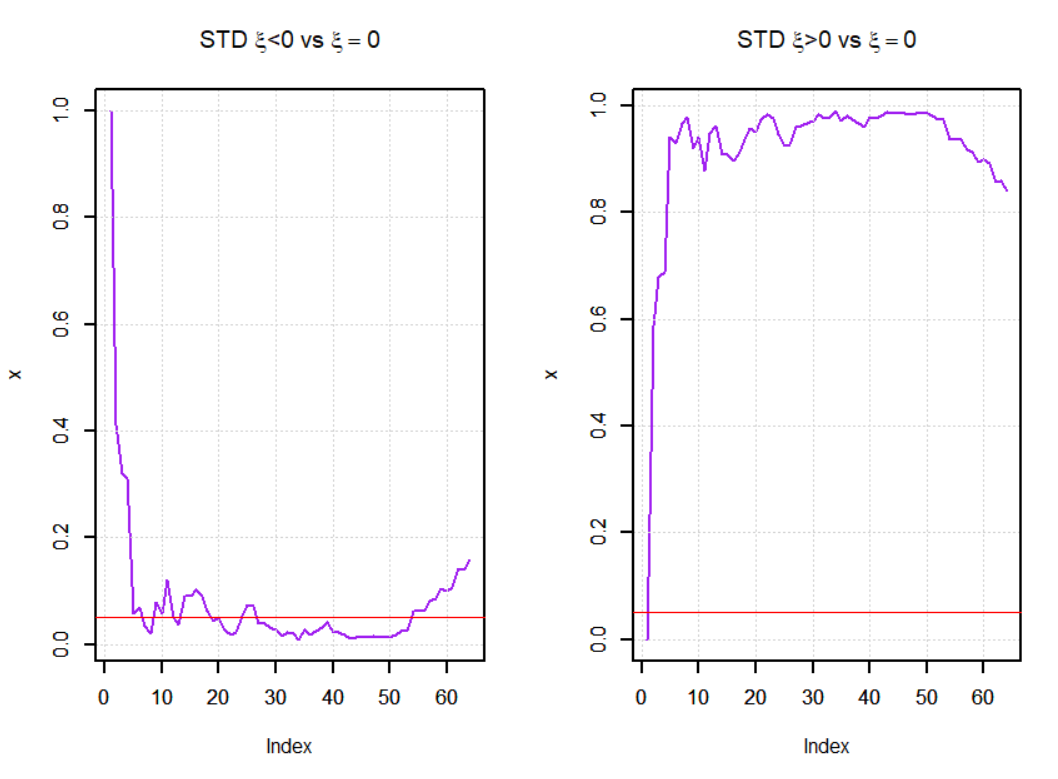
\includegraphics[scale = 0.5]{PH1.png}
\caption{Prueba de Hipótesis \(G_{n,k}(0)\) vista en ayudantía: \(\xi <0\) vs \(\xi = 0\).}
    \label{fig:13}
\end{figure}

%%%%%%%%%%%%%%%%%%%%%%%%%%%%%%%%%%%%%%%%%%%%%%%%%%%%%%%%%%%%%%%%%%%%%%%%%%%%%%%%% Pertenencia dom de atracción minimos. 
\begin{figure}[htb]
    \centering
    \includegraphics[scale = 0.5]{Fep2.png}
    \caption{FEP's empíricas de los datos en negativos.}
    \label{fig:2/2}
\end{figure}

\begin{figure}[htb]
    \centering
    \includegraphics[scale = 0.5]{FepCoc2.png}
    \caption{Cocientes FEP empíricos de los datos en negativo.}
    \label{fig:2/3}
\end{figure}

\begin{figure}[htb]
    \centering
    \includegraphics[scale = 0.5]{FepCoc2Zoom.png}
    \caption{Cocientes FEP empíricos con Zoom de los datos en negativo.}
    \label{fig:2/4}
\end{figure}

\begin{figure}[htb]
    \centering
    \includegraphics[scale = 0.5]{FepTrans2.png}
    \caption{FEP's empíricas de los datos negativos transformados.}
    \label{fig:2/5}
\end{figure}

\begin{figure}[htb]
    \centering
    \includegraphics[scale = 0.5]{FepCocTrans2.png}
    \caption{Cocientes FEP empíricos de los datos negativos transformados.}
    \label{fig:2/6}
\end{figure}

\begin{figure}[htb]
    \centering
    \includegraphics[scale = 0.5]{FepCocTrans21.png}
    \caption{Cocientes FEP empíricos de los datos negativos transformados. Zoom para Enero, Febrero, Marzo y Abril dejando a la cola menos del \(8\%\) de los datos, i.e, entre 8 y 9 datos.}
    \label{fig:2/6.1}
\end{figure}

\begin{figure}[htb]
    \centering
    \includegraphics[scale = 0.5]{FepCocTrans22.png}
    \caption{Cocientes FEP empíricos de los datos negativos transformados. Zoom para Mayo, Junio, Julio y Agosto dejando a la cola menos del \(8\%\) de los datos, i.e, entre 8 y 9 datos.}
    \label{fig:2/6.2}
\end{figure}

\begin{figure}[htb]
    \centering
    \includegraphics[scale = 0.5]{FepCocTrans23.png}
    \caption{Cocientes FEP empíricos de los datos negativos transformados. Zoom para Septiembre, Octubre, Noviembre y Diciembre dejando a la cola menos del \(8\%\) de los datos, i.e, entre 8 y 9 datos.}
    \label{fig:2/6.3}
\end{figure}

\begin{figure}[htb]
    \centering
    \includegraphics[scale = 0.5]{ENEFEB2.png}
    \caption{Parámetros DGP Ajustada a mínimos de máximos Enero: \(\xi = -0.550\), \(a(u)=4.575\) y \(u = -45.9\). Parámetros DGP Ajustada a mínimos de máximos febrero: \(\xi =-0.375\), \(a(u)=5.224\) y \(u= -45.75\).}
    \label{fig:2/7}
\end{figure}  


\begin{figure}[htb]
    \centering
    \includegraphics[scale = 0.5]{MARAPR2.png}
    \caption{Parámetros DGP Ajustada a mínimos de máximos marzo: \(\xi =  -0.700\), \(a(u)=8.223\) y \(u = -59.3\). Parámetros DGP Ajustada a mínimos de máximos abril: \(\xi =  -0.733\), \(a(u)=  5.824\) y \(u = -74.7\).}
    \label{fig:2/8}
\end{figure} 


\begin{figure}[htb]
    \centering
    \includegraphics[scale = 0.5]{MAYJUN2.png}
    \caption{Parámetros DGP Ajustada a mínimos de máximos mayo: \(\xi =-0.620\), \(a(u)=5.682\) y \(u = -83.6\). Parámetros DGP Ajustada a mínimos de máximos junio: \(\xi =-0.133\), \(a(u)=2.495\) y \(u = -89.18\).}
    \label{fig:2/9}  
\end{figure} 


\begin{figure}[htb]
    \centering
    \includegraphics[scale = 0.5]{JUlAUG2.png}
    \caption{Parámetros DGP Ajustada a mínimos de máximos julio: \(\xi = -0.294\), \(a(u)=3.101 \) y \(u =-91.65\). Parámetros DGP Ajustada a mínimos de máximos agosto: \(\xi = -0.297\), \(a(u)=2.177\) y \(u =  -88.7\).}
    \label{fig:2/10}    
\end{figure} 

5.002 
\begin{figure}[htb]
    \centering
    \includegraphics[scale = 0.5]{SEPOCT2.png}
    \caption{Parámetros DGP Ajustada a mínimos de máximos septiembre: \(\xi =  -1.056\), \(a(u)= 5.002 \) y \(u =-84.6\). Parámetros DGP Ajustada a mínimos de máximos octubre: \(\xi = -0.292\), \(a(u)=2.783 \) y \(u = -75.4\).}
    \label{fig:2/11}
\end{figure} 


\begin{figure}[htb]
    \centering
    \includegraphics[scale = 0.5]{DEC.png}
    \caption{Parámetros DGP Ajustada a mínimos de máximos diciembre: \(\xi =-0.546\), \(a(u)=6.132\) y \(u =-49.6\).}
    \label{fig:2/12}
\end{figure}


\begin{figure}[htb]
    \centering
    \includegraphics[scale = 0.5]{PH2.png}
    \caption{Prueba de Hipótesis \(G_{n,k}(0)\) vista en ayudantía: \(\xi <0\) vs \(\xi = 0\).}
    \label{fig:2/13}
\end{figure}

%%%%%%%%%%%%%%%%%%%%%%%%%%%%%%%%%%%%%%%%%%%%%%%%%%%%%%%%%%%%%%%%%%%%%%%%Extremos derechos

\begin{figure}[htb]
    \centering
    \includegraphics[scale = 0.5]{MAyu1.png}
    \caption{Gráficas de la metodología vista en la ayudantía para la estimación del extremo derecho: Metodología aplicada a las distribuciones de los datos de máximos de temperaturas, para aquellos meses indicados en los títulos de las gráficas. }
    \label{fig:20}
\end{figure}

\begin{figure}[htb]
    \centering
    \includegraphics[scale = 0.5]{MAyu12.png}
    \caption{Gráficas de la metodología vista en la ayudantía para la estimación del extremo derecho: Metodología aplicada a las distribuciones de los datos de máximos de temperaturas, para aquellos meses indicados en los títulos de las gráficas. }
    \label{fig:21}
\end{figure}

\begin{figure}[htb]
    \centering
    \includegraphics[scale = 0.5]{MAyu13.png}
    \caption{Gráficas de la metodología vista en la ayudantía para la estimación del extremo derecho: Metodología aplicada a las distribuciones de los datos de máximos de temperaturas, para aquellos meses indicados en los títulos de las gráficas. }
    \label{fig:22}
\end{figure}

\begin{figure}[htb]
    \centering
    \includegraphics[scale = 0.5]{MAyu21.png}
    \caption{Gráficas de la metodología vista en la ayudantía para la estimación del extremo derecho: Metodología aplicada a las distribuciones del negativo de los datos de máximos de temperaturas, para aquellos meses indicados en los títulos de las gráficas. }
    \label{fig:23}
\end{figure}

\begin{figure}[htb]
    \centering
    \includegraphics[scale = 0.5]{MAyu22.png}
    \caption{Gráficas de la metodología vista en la ayudantía para la estimación del extremo derecho: Metodología aplicada a las distribuciones del negativo de los datos de máximos de temperaturas, para aquellos meses indicados en los títulos de las gráficas. }
    \label{fig:24}
\end{figure}

\begin{figure}[htb]
    \centering
    \includegraphics[scale = 0.5]{MAyu23.png}
    \caption{Gráficas de la metodología vista en la ayudantía para la estimación del extremo derecho: Metodología aplicada a las distribuciones del negativo de los datos de máximos de temperaturas, para aquellos meses indicados en los títulos de las gráficas. }
    \label{fig:25}
\end{figure}





















\newpage

\end{document}


\begin{figure}[h]
    \centering
    \includegraphics[width=0.6\textwidth]{Ej2eFEP.png}
    \caption{FEP empírica de las muestras conjuntas de los meses}
    \label{Ej2eFEP}
\end{figure}

\begin{figure}[h]
    \centering
    \includegraphics[width=0.6\textwidth]{Ej2eCFEP.png}
    \caption{Cociente FEP empírico de las muestras conjuntas de los meses}
    \label{Ej2eCFEP}
\end{figure}
\begin{figure}[h]
    \centering
    \includegraphics[width=0.6\textwidth]{Imagenes finales/Ej2eCFEPzoom.png}
    \caption{Cociente FEP empírico de las muestras conjuntas de los meses}
    \label{Ej2eCFEPZoom}
\end{figure}

\begin{figure}[h]
    \centering
    \includegraphics[width=0.6\textwidth]{Imagenes finales/FEPPTra.png}
    \caption{Fep empírica de las muestras conjuntas de datos transformados}
    \label{Ej2eCFEPtrans}
\end{figure}

\begin{figure}[h]
    \centering
    \includegraphics[width=0.6\textwidth]{Ej2eCFEPtrans.png}
    \caption{Cociente Fep empírico de las muestras conjuntas de datos transformados}
    \label{ZEj2eCFEPtransZ}
\end{figure}


\begin{figure}[htb]
    \centering
    \includegraphics[scale = 0.7]{Imagenes finales/AjustePareto.png}
    \caption{Parámetros de la DGP Ajustada a Grupo 1 de datos originales \(\xi =-0.16\), \(a(u)=4.61\) y \(u = 60.3\). Parámetros de la DGP Ajustada a Grupo 2 de datos originales: \(\xi = -0.160\), \(a(u)=2.449\) y \(u = 92.25\).  Parámetros de la DGP Ajustada a Grupo 3 de datos originales: \(\xi =-0.342 \), \(a(u)=-2.460 \) y \(u = 96.2\).}
    \label{Mon1DGP} 
\end{figure}

\begin{comment}
%%%%%%%%%%%%%%%%%%%%%%%%%%%%%%%%%%%%%%5555Termina bondad y ajuste máximos de máximo inicia mínimos de máximos 
\begin{figure}[h]
    \centering
    \includegraphics[width=0.6\textwidth]{.png}
    \caption{FEP empírica de las muestras conjuntas de los meses. Datos negativos.}
    \label{mEj2eFEP}
\end{figure}
\begin{figure}[h]
    \centering
    \includegraphics[width=0.6\textwidth]{}
    \caption{Cociente FEP empírico de las muestras conjuntas de los meses. Datos negativos.}
    \label{mEj2eCFEP}
\end{figure}


\begin{figure}[h]
    \centering
    \includegraphics[width=0.6\textwidth]{.png}
    \caption{FEP empírico de las muestras conjuntas de los meses. Datos negativos.}
    \label{mEj2eCFEPZoom}
\end{figure}

\begin{figure}[h]
    \centering
    \includegraphics[width=0.6\textwidth]{.png}
    \caption{Cociente Fep empírico de las muestras conjuntas de datos transformados. Datos negativos.}
    \label{mEj2eCFEPtrans}
\end{figure}


\begin{figure}[htb]
    \centering
    \includegraphics[scale = 0.5]{.png}
    \caption{Parámetros de la DGP Ajustada a Grupo 1 de datos negativos \(\xi =-0.16\), \(a(u)=4.61\) y \(u = 60.3\). Parámetros de la DGP Ajustada a Grupo 2 de datos negativos: \(\xi = -0.160\), \(a(u)=2.449\) y \(u = 92.25\).  Parámetros de la DGP Ajustada a Grupo 3 de datos negativos: \(\xi =-0.342 \), \(a(u)=-2.460 \) y \(u = 96.2\). Datos negativos.}
    \label{mMon1DGP} 
\end{figure}
\end{comment}

%%%%%%%%%%%%%%%%%%%%%%%%%%%%%%%%%%%%%%%%%%% Ext derechos max de max
\begin{figure}[htb]
    \centering
    \includegraphics[scale = 0.5]{Imagenes finales/ExtremoderechoMax.png}
    \caption{Estimaciones de los extremos derechos, mediante la metodología vista en la ayudantía. Las estimaciones corresponden a los extremos derechos de \(F_1, F_2\) y \(F_3\) de manera respectivamente.}
    \label{ExtDerDGP} 
\end{figure}
%%%%%%%%%%%%%%%%%%%%%%%%%%%%%%%%%%%%%%%%%%% Ext  izquierdos max de max
\begin{figure}[htb]
    \centering
    \includegraphics[scale = 0.6]{Imagenes finales/ExtremoderNeg.png}
    \caption{Estimaciones de los extremos derechos, mediante la metodología vista en la ayudantía. Las estimaciones corresponden a los extremos derechos de \(G_1, G_2\) y \(G_3\) de manera respectiva. Datos negativos.}
    \label{mExtDerDGP} 
\end{figure}
%%%%%%%%%%%%%%%%%%%%%%%%%%%%%%%%%%%%%%%%%%%%%%%%%%%%%%%%%%%%%datosnega
\begin{figure}[htb]
    \centering
    \includegraphics[scale = 0.6]{Imagenes finales/FEPneg.png}
    \caption{FEP's empíricas de los datos en negativo.}
    \label{mEj2eFEP} 
\end{figure}
\begin{figure}[htb]
    \centering
    \includegraphics[scale = 0.6]{Imagenes finales/CFEPneg.png}
    \caption{Cocientes FEP empíricos de los datos en negativo.}
    \label{mEj2eCFEP} 
\end{figure}
\begin{figure}[htb]
    \centering
    \includegraphics[scale = 0.6]{Imagenes finales/CFEPnegzoom.png}
    \caption{Cocientes FEP empíricos de los datos con Zoom negativo.}
    \label{mEj2eCFEPZoom} 
\end{figure}
\begin{figure}[htb]
    \centering
    \includegraphics[scale = 0.6]{Imagenes finales/FEPneg.png}
    \caption{FEP's empíricos de los datos tranformados.}
    \label{mEj2eFEPtrans} 
\end{figure}
%\begin{figure}[htb]
%    \centering
%    \includegraphics[scale = 0.6]{Ej2eCFEP.png}
%    \caption{Cociente FEP empíricos de los datos tranformados.}
%    \label{mEj2eCFEPtrans} 
%\end{figure}






